%%%%%%%%%%%%%%%%%%%%%%%%%%%%%%%%%%%%%%%%%
% Proceedings of the National Academy of Sciences (PNAS)
% LaTeX Template
% Version 1.0 (19/5/13)
%
% This template has been downloaded from:
% http://www.LaTeXTemplates.com
%
% Original author:
% The PNAStwo class was created and is owned by PNAS:
% http://www.pnas.org/site/authors/LaTex.xhtml
% This template has been modified from the blank PNAS template to include
% examples of how to insert content and drastically change commenting. The
% structural integrity is maintained as in the original blank template.
%
% Original header:
%% PNAStmpl.tex
%% Template file to use for PNAS articles prepared in LaTeX
%% Version: Apr 14, 2008
%
%%%%%%%%%%%%%%%%%%%%%%%%%%%%%%%%%%%%%%%%%
%----------------------------------------------------------------------------------------
%	PACKAGES AND OTHER DOCUMENT CONFIGURATIONS
%----------------------------------------------------------------------------------------

%------------------------------------------------
% BASIC CLASS FILE
%------------------------------------------------

%% PNAStwo for two column articles is called by default.
%% Uncomment PNASone for single column articles. One column class
%% and style files are available upon request from pnas@nas.edu.

%\documentclass{pnasone}
\documentclass{pnastwo}

%------------------------------------------------
% POSITION OF TEXT
%------------------------------------------------

%% Changing position of text on physical page:
%% Since not all printers position
%% the printed page in the same place on the physical page,
%% you can change the position yourself here, if you need to:

% \advance\voffset -.5in % Minus dimension will raise the printed page on the 
                         %  physical page; positive dimension will lower it.

%% You may set the dimension to the size that you need.

%------------------------------------------------
% GRAPHICS STYLE FILE
%------------------------------------------------

%% Requires graphics style file (graphicx.sty), used for inserting
%% .eps/image files into LaTeX articles.
%% Note that inclusion of .eps files is for your reference only;
%% when submitting to PNAS please submit figures separately.

%% Type into the square brackets the name of the driver program 
%% that you are using. If you don't know, try dvips, which is the
%% most common PC driver, or textures for the Mac. These are the options:

% [dvips], [xdvi], [dvipdf], [dvipdfm], [dvipdfmx], [pdftex], [dvipsone],
% [dviwindo], [emtex], [dviwin], [pctexps], [pctexwin], [pctexhp], [pctex32],
% [truetex], [tcidvi], [vtex], [oztex], [textures], [xetex]


%------------------------------------------------
% OPTIONAL POSTSCRIPT FONT FILES
%------------------------------------------------

%% PostScript font files: You may need to edit the PNASoneF.sty
%% or PNAStwoF.sty file to make the font names match those on your system. 
%% Alternatively, you can leave the font style file commands commented out
%% and typeset your article using the default Computer Modern 
%% fonts (recommended). If accepted, your article will be typeset
%% at PNAS using PostScript fonts.

% Choose PNASoneF for one column; PNAStwoF for two column:
%\usepackage{PNASoneF}
%\usepackage{PNAStwoF}

%------------------------------------------------
% ADDITIONAL OPTIONAL STYLE FILES
%------------------------------------------------

%% The AMS math files are commonly used to gain access to useful features
%% like extended math fonts and math commands.
\usepackage{multirow}
%\usepackage{caption}
%\usepackage{subcaption}
\usepackage{etex}
\usepackage{color}
%\usepackage[usenames,dvipsnames,svgnames,table]{xcolor}
%\usepackage[usenames,dvipsnames]{xcolor}
\usepackage{tikz}
\usetikzlibrary{decorations.shapes}
\usepackage{amssymb,amsfonts,amsmath}
\usepackage{xspace}
\newcommand{\dictionary}{\ensuremath{\mathcal{D}}\xspace}
\usepackage{soul}
%\usepackage{hyperref}

%------------------------------------------------
% OPTIONAL MACRO FILES
%------------------------------------------------

%% Insert self-defined macros here.
%% \newcommand definitions are recommended; \def definitions are supported

%\newcommand{\mfrac}[2]{\frac{\displaystyle #1}{\displaystyle #2}}
%\def\s{\sigma}

%------------------------------------------------
% DO NOT EDIT THIS SECTION
%------------------------------------------------

%% For PNAS Only:
\contributor{Submitted to Proceedings of the National Academy of Sciences of the United States of America}
\url{www.pnas.org/cgi/doi/10.1073/pnas.0709640104}
\copyrightyear{2008}
\issuedate{Issue Date}
\volume{Volume}
\issuenumber{Issue Number}

%----------------------------------------------------------------------------------------

\begin{document}

%----------------------------------------------------------------------------------------
%	TITLE AND AUTHORS
%----------------------------------------------------------------------------------------

\title{Nonliteral understanding of number words} % For titles, only capitalize the first letter

%------------------------------------------------

%% Enter authors via the \author command.  
%% Use \affil to define affiliations.
%% (Leave no spaces between author name and \affil command)

%% Note that the \thanks{} command has been disabled in favor of
%% a generic, reserved space for PNAS publication footnotes.

%% \author{<author name>
%% \affil{<number>}{<Institution>}} One number for each institution.
%% The same number should be used for authors that
%% are affiliated with the same institution, after the first time
%% only the number is needed, ie, \affil{number}{text}, \affil{number}{}
%% Then, before last author ...
%% \and
%% \author{<author name>
%% \affil{<number>}{}}

%% For example, assuming Garcia and Sonnery are both affiliated with
%% Universidad de Murcia:
%% \author{Roberta Graff\affil{1}{University of Cambridge, Cambridge,
%% United Kingdom},
%% Javier de Ruiz Garcia\affil{2}{Universidad de Murcia, Bioquimica y Biologia
%% Molecular, Murcia, Spain}, \and Franklin Sonnery\affil{2}{}}

\author{Justine T. Kao\affil{1}{Stanford University},
Jean Wu,\affil{1}{}
Leon Bergen\affil{2}{MIT}
\and
Noah D. Goodman\affil{1}{}}

\contributor{Submitted to Proceedings of the National Academy of Sciences
of the United States of America}

%----------------------------------------------------------------------------------------

\maketitle % The \maketitle command is necessary to build the title page

\begin{article}

%----------------------------------------------------------------------------------------
%	ABSTRACT, KEYWORDS AND ABBREVIATIONS
%----------------------------------------------------------------------------------------

\begin{abstract}
One of the most puzzling and important facts about communication is that people do not always mean what they say; speakers often use imprecise, exaggerated, or otherwise literally false descriptions to communicate experiences and opinions. Here we focus on the nonliteral interpretation of number words, in particular hyperbole (interpreting unlikely numbers as exaggerated and conveying affect) and pragmatic halo (interpreting round numbers imprecisely). We provide a computational model of number interpretation as social inference regarding the communicative goal, meaning, and affective subtext of an utterance. We show that our model predicts humans' interpretation of number words with high accuracy. Our model is the first computational model that quantitatively predicts hyperbolic and pragmatic halo effects in number interpretation using a unified framework. 
This modeling framework provides an approach to nonliteral language understanding more generally.
\end{abstract}

%------------------------------------------------

\keywords{Pragmatics | Language understanding | Computational modeling} % When adding keywords, separate each term with a straight line: |

%------------------------------------------------

%% Optional for entering abbreviations, separate the abbreviation from
%% its definition with a comma, separate each pair with a semicolon:
%% for example:
%% \abbreviations{SAM, self-assembled monolayer; OTS,
%% octadecyltrichlorosilane}

% \abbreviations{}
%\abbreviations{IR, Incongruity Resolution}

%----------------------------------------------------------------------------------------
%	PUBLICATION CONTENT
%----------------------------------------------------------------------------------------

%% The first letter of the article should be drop cap: \dropcap{} e.g.,
%\dropcap{I}n this article we study the evolution of ''almost-sharp'' fronts

\section{Introduction}

\dropcap{I}magine a friend describing a new restaurant where she recently dined. Your friend says, ``It took 30 minutes to get a table." You are likely to interpret this to mean she waited approximately 30 minutes. Suppose she says: ``It took 32 minutes to get a table." You are more likely to interpret this to mean exactly 32 minutes. Now, suppose she says: ``It took a million years to get a table." You will probably interpret this to mean that the wait was shorter than a million years, but importantly that she thinks it took much too long. One of the most fascinating facts about communication is that people do not always mean what they say---a crucial part of the listener's job is to understand an utterance even when its literal meaning is false. People's ability to interpret nonliteral language poses a critical puzzle for research on language understanding.

% Some sentences very similar to cogsci paper.
A rich body of literature in psychology and linguistics has examined how people use and understand nonliteral language \cite{roberts1994, dews1999, glucksberg2001, gibbs1999}. However, much of the work has been qualitative, with little focus on analyzing aspects of an utterance that predict the quantitative details of people's figurative interpretations. Here we present a model that formalizes and integrates three general principals of language and communication to explain the computational basis of nonliteral language understanding. First, speakers and listeners communicate with the assumption that their interlocutors are rational and cooperative agents; second, listeners assume that speakers choose utterances to maximize informativeness with respect to their communicative goals; third, speaker and listener utilize common ground---their shared knowledge of the world---to communicate effectively. These ideas have important connections to Gricean pragmatics \cite{grice1975, clark1996} and relevance theory \cite{relevance,wilson2002}. 
For instance, proponents of relevance theory argue that listeners infer the meaning of a metaphor, as well as other forms of loose talk, by assuming that speakers maximize relevance \cite{sperber2008, wilson2006, loosetalk}. 
Here we formalize the notion that speakers have a goal to maximize informativeness about a given topic. By applying this computational approach to a case study on number words, we show that nonliteral interpretations can arise from principles of communication without positing dedicated processing mechanisms for nonliteral language.

A recent body of work has formalized communication as an interaction between rational and cooperative agents. These Rational Speech Act (RSA) models view pragmatic language understanding as probabilistic inference over recursive social models and are able to quantitatively explain a range of phenomena in human pragmatic reasoning \cite{frankgoodmanscience, goodmanstuhlmueller, bergen2012, jager2009pragmatic}. At the core of these models, a listener and a speaker recursively reason about each other to arrive at pragmatically enriched meanings. Given an intended meaning $m$, speaker $S_n$ reasons about listener $L_{n-1}$ and chooses utterance $u$ based on the probability that the listener will successfully infer the intended meaning \cite{bergen2012}:
$$
S_n (u|m) \propto L_{n-1} (m|u) \cdot e^{-C(u)}
$$

The listener $L_n$ then reasons about $S_n$ and uses Bayes' Rule to infer the meaning $m$ given utterance $u$:
$$
L_n (m|u) \propto P(m)S_n (u|m)
$$
%The recursion begins with a na�ve listener, $L_0$, who interprets $u$ literally.
The RSA framework predicts that it is never optimal for a speaker to choose an utterance whose literal meaning directly contradicts her intended meaning. However, this contradictory use is precisely the case in nonliteral language. For example, ``It took a million years to get a table" conveys that the wait time was long but not, in fact, a million years. This suggests that the basic RSA model is incomplete and requires additional elements to explain nonliteral communication.

Previous work has examined people's communicative reasons for using figurative language and suggested that certain goals, such as conveying emotion and emphasis, are best satisfied by nonliteral language \cite{roberts1994}. Here we propose that language understanding in general, and nonliteral language understanding in particular, relies on reasoning about communicative goals during interpretation. We introduce a model in which the listener is uncertain about the speaker's communicative goal and performs joint inference on both the goal and the intended meaning. Importantly, the interpretation space has multiple dimensions, and different communicative goals are satisfied by different aspects of the inferred meaning. A speaker's goal may be to maximize the probability of successfully conveying information along one dimension of meaning but not another, which makes it possible for a literally false utterance to be optimal as long as it is informative along the target dimension. We explore the case where the interpretation space has two dimensions: the state of the world (e.g.~the true amount) and the speaker's affect or opinion\footnote{In what follows we describe the subtext dimension as ``affect,'' but it could be other kinds of speaker opinion, \emph{mutatis mutandis}.}. The speaker is now modeled as: \hl{fixed}
$$
S_n(u | s, a, g) \propto \sum_{s', a'}\delta_{g(s,a)=g(s',a')}L_n(s',a'|u)\cdot e^{-c(u)}
$$
where the intended meaning includes $s$ (the state of the world) and  $a$ (the speaker's affect). $g$ is a function that projects the listener's inferred meaning onto dimensions that are relevant to the speaker's communicative goal, and $C$ is a function for utterance costs. A literal listener interprets utterances literally without reasoning about the speaker, while a pragmatic listener performs joint inference on both the speaker's goal and her intended meaning (see Materials):
$$
L_n (s,a | u) \propto \sum_g P_S(s) P_A(a|s) P_G(g|s,a) S_{n-1} (u|g)
$$
The listener utilizes prior knowledge of the probability of a state ($P_S$) and the probability of having a particular affect given a state ($P_A$). 
The literal meaning of utterance $u$ may convey nothing about the affective subtext $a$; it conveys information about the state $s$. However, the common knowledge that affect is usually associated with certain states of the world allows the speaker to use an assertion that the state is $s$ to convey the corresponding information about $a$. If it is known that the goal is to convey affect, and not the state, then the pragmatic listener will discount the information about $s$ but retain the information about $a$---a nonliteral interpretation is obtained.
Even when the pragmatic listener is not certain of the speaker's goal, a joint inference of goal, state, and affect results in the same nonliteral interpretation.
Common knowledge of a domain and joint reasoning about communicative goals thus allows the speaker to communicate additional dimensions of meaning, such as affect, without explicitly describing these dimensions.

This formulation of language understanding as joint inference of the communicative goal, state of the world, and affective subtext of an utterance provides a computational approach extending the RSA framework to nonliteral language understanding. As a case study, we focus on the nonliteral interpretation of number words. We chose number words because they have precise literal meanings that can be easily modeled, and apply to domains (such as prices) that lend themselves to quantitative measurement.
%, whereas the literal meanings of concepts such as \hl{``Juliet" and ``the sun" }are more difficult to formalize. 
We aim to capture two particular well-known phenomena regarding number interpretation: hyperbole and pragmatic halo. Hyperbole is a figure of speech that uses exaggeration to convey emphasis and emotion \cite{mccarthy2004there}. While hyperbolic utterances are literally false, such indirect communication is readily understood and serves many purposes \cite{roberts1994, mccarthy2004there, gibbs2000irony, gibbs1991}. Pragmatic halo refers to people's tendency to interpret round numbers such as $100$ imprecisely and complex numbers such as $103$ precisely \cite{lasersohn1999}. The halo effect has been formalized in game theoretic models as a rational choice given different utterance costs and a possibility of pragmatic slack \cite{bastiaanse2011rationality, krifka2007approximate}. Other research has shown that speakers' tendency to choose simple number expressions decreases when more precise information is relevant to the listener \cite{vanderhest2002}. This suggests that higher-level pragmatic considerations such as communicative goals directly impact the production and interpretation of round versus sharp numbers. Our model uses alternative communicative goals coupled with differential utterance costs to model the pragmatic halo effect. We show that our framework for pragmatic inference makes quantitative predictions for both hyperbole and pragmatic halo in the interpretation of number words.
%------------------------------------------------

\section{Results}

%Given that knowledge of a domain's prior distribution drives hyperbolic interpretations, we predict that the same number word used in different domains will elicit different interpretations.
We tested our model on number words that refer to the prices of three types of everyday items: electric kettles, watches, and laptops. We selected these items because they have distinct price distributions, the prior $P_S$, which we measured empirically by asking participants to rate the probability of various prices for the three items (see Experiment 3a in Methods). We also obtained an affect prior, $P_A$, by asking participants to rate the probability of a speaker thinking that an item is too expensive given a price state (see Experiment 3b). \hl{fixed} Given these priors, we aimed to model people's interpretations of utterances such as, ``The electric kettle cost $u$ dollars," for $u \in U$, assuming that a listener can interpret this utterance to mean that the kettle cost $s$ dollars, for $s \in S$. We selected $U$ such that each number word is either ``round" (divisible by 10 and less costly to utter) or ``sharp" (not divisible by 10 and more costly to utter). A formal description of these assumptions is in the Methods section.

\begin{figure}[t]
\centering
\begin{minipage}[b]{.49\textwidth}
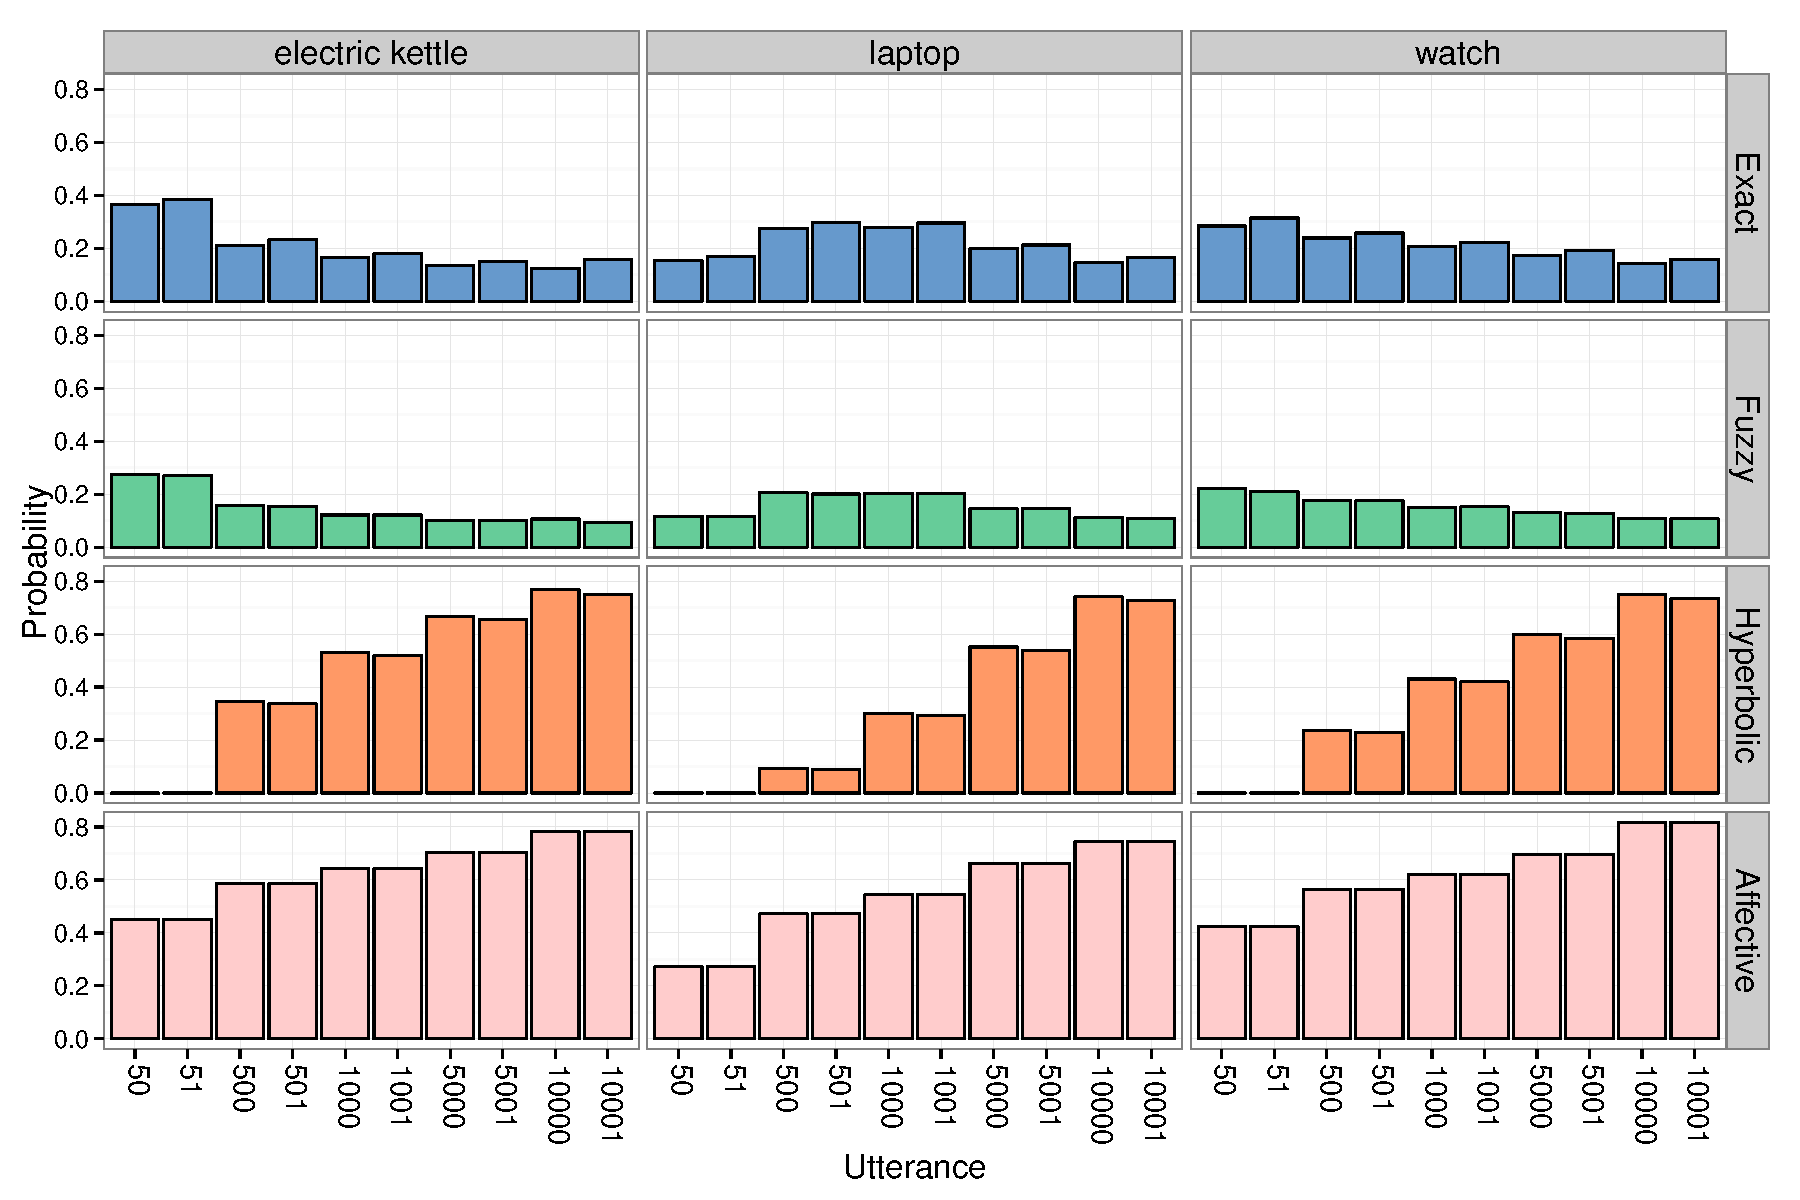
\includegraphics[width=8.7cm]{model_effects.pdf}
\caption{Each vertical panel column shows the probabilities of different kinds of interpretations given utterances about an item (see text).}\label{model_effects}
\end{minipage}\hfill
\end{figure}

\begin{figure*}
\centering
\begin{minipage}[b]{.49\textwidth}
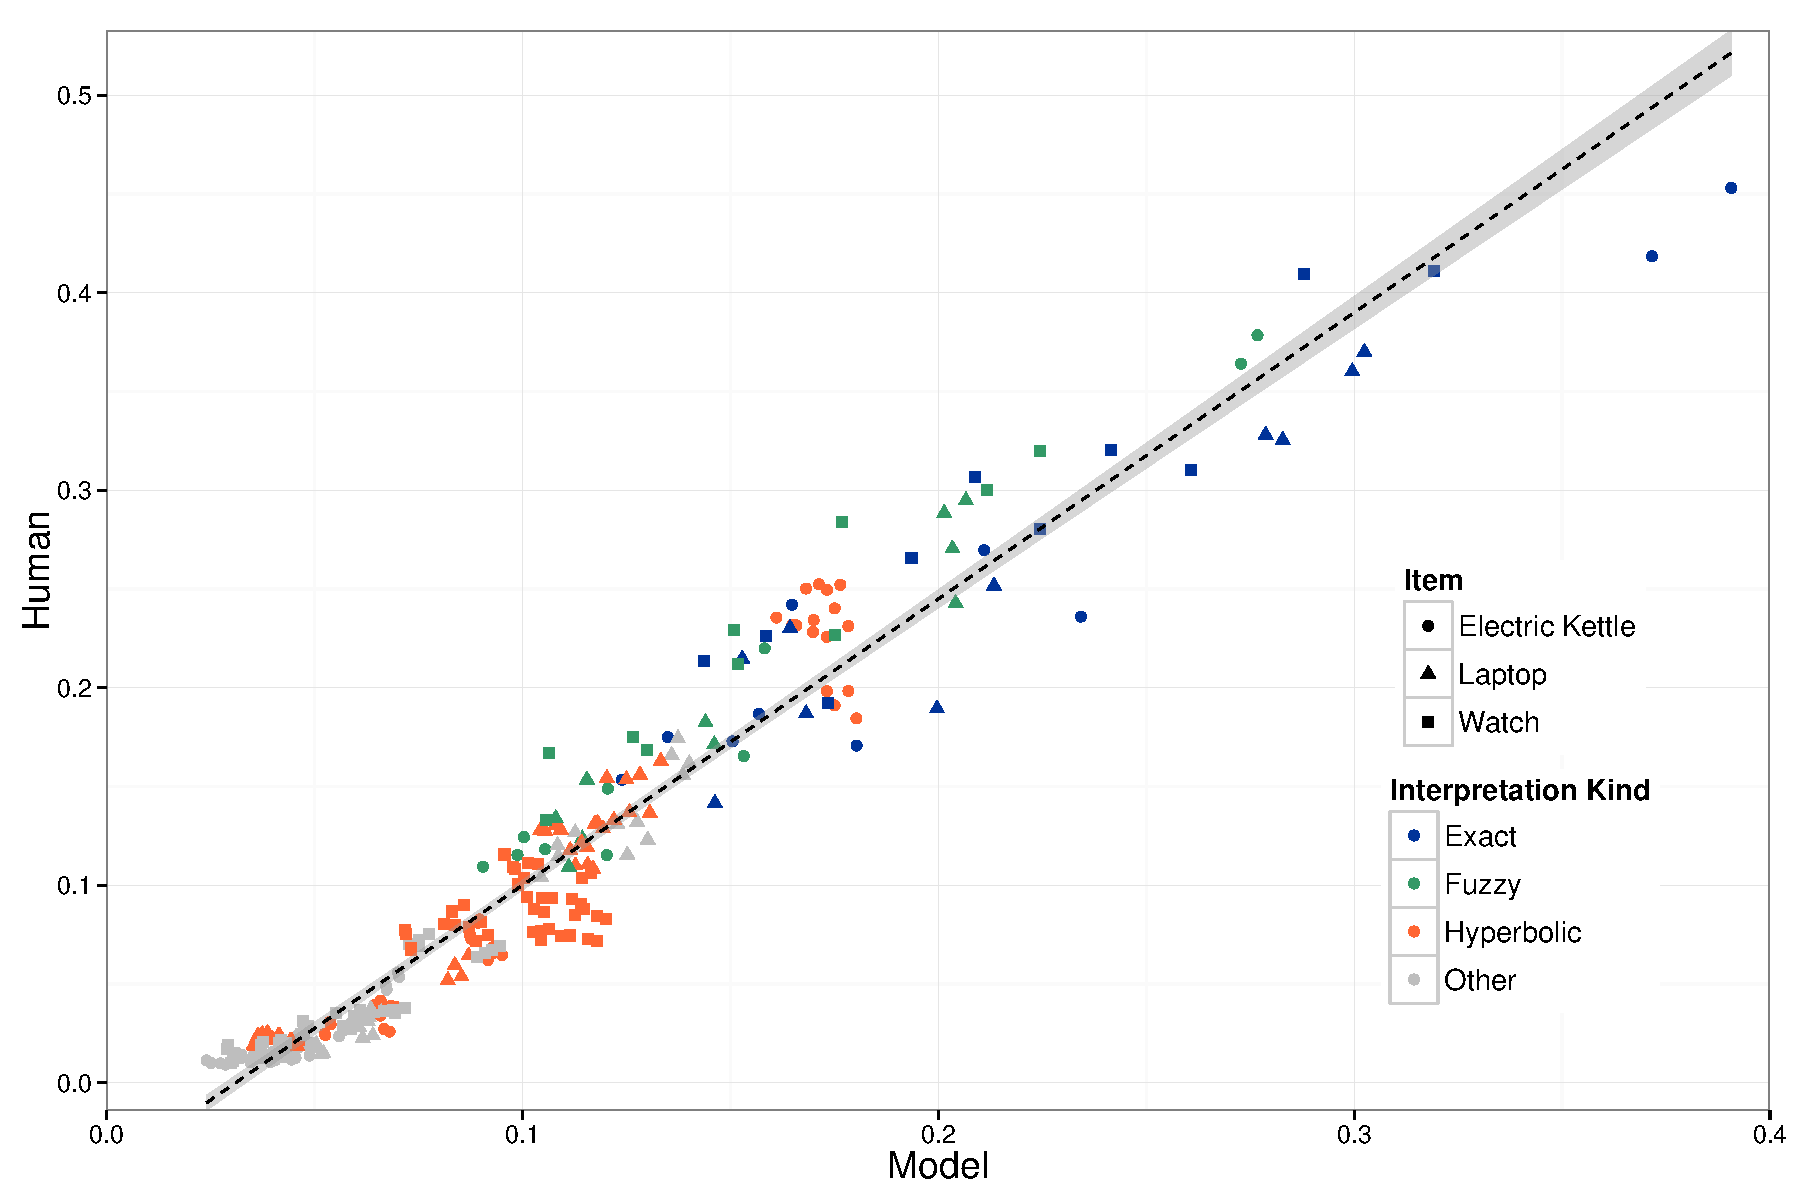
\includegraphics[width=8.7cm]{model_human_scatter.pdf}
\caption{Hello}
\end{minipage}
\begin{minipage}[b]{.49\textwidth}
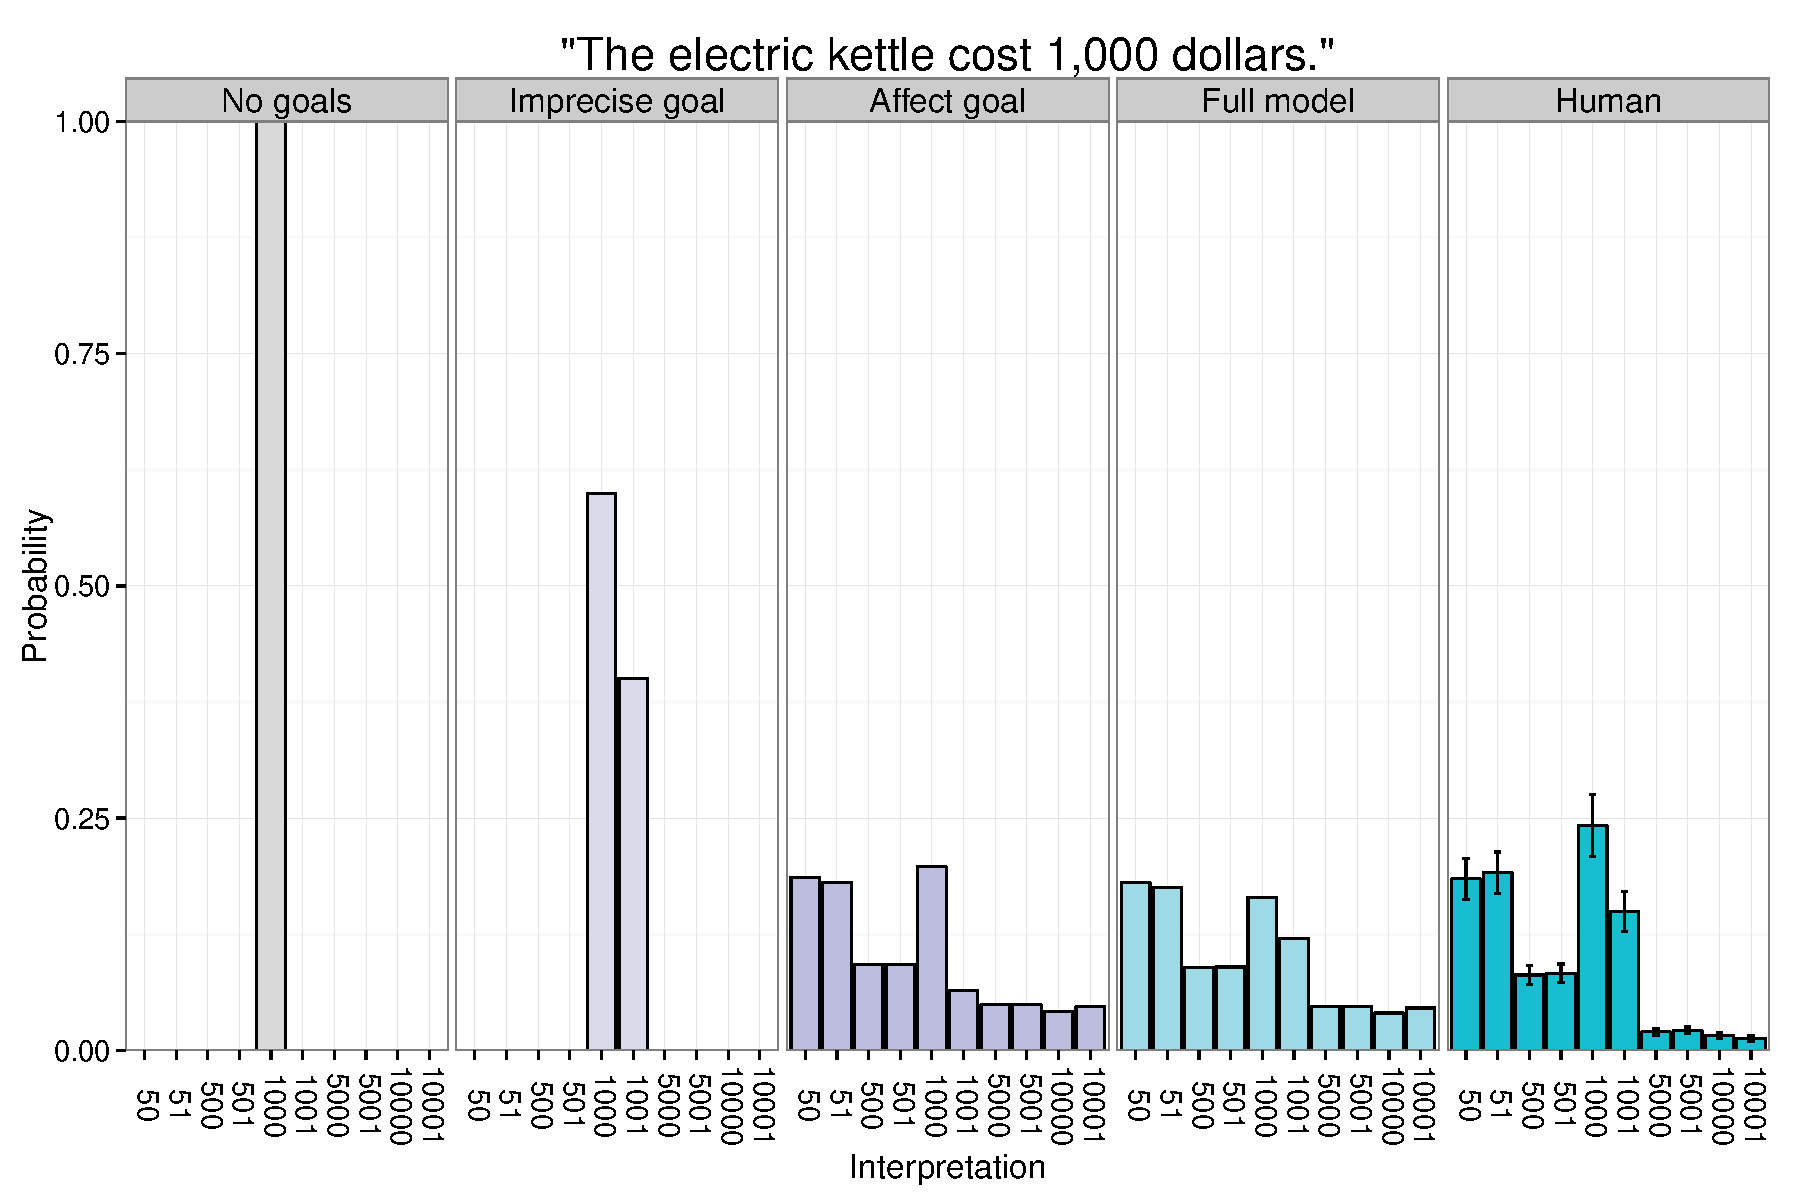
\includegraphics[width=8.7cm]{model_comp_goals.pdf}
\caption{(A) Model predictions (x-axis) versus average human responses (y-axis) for 300 data points (3 Items $\times$ 10 Utterances $\times$ 10 Price States) in Experiment 1. (B) Human interpretations of a sample utterance and model predictions given different communicative goals. A model that considers both affect and precision goals closely matches human data.}
\end{minipage}\hfill
\label{model_fit_and_halo}
\end{figure*}

\begin{figure*}

\begin{minipage}[b]{.49\textwidth}
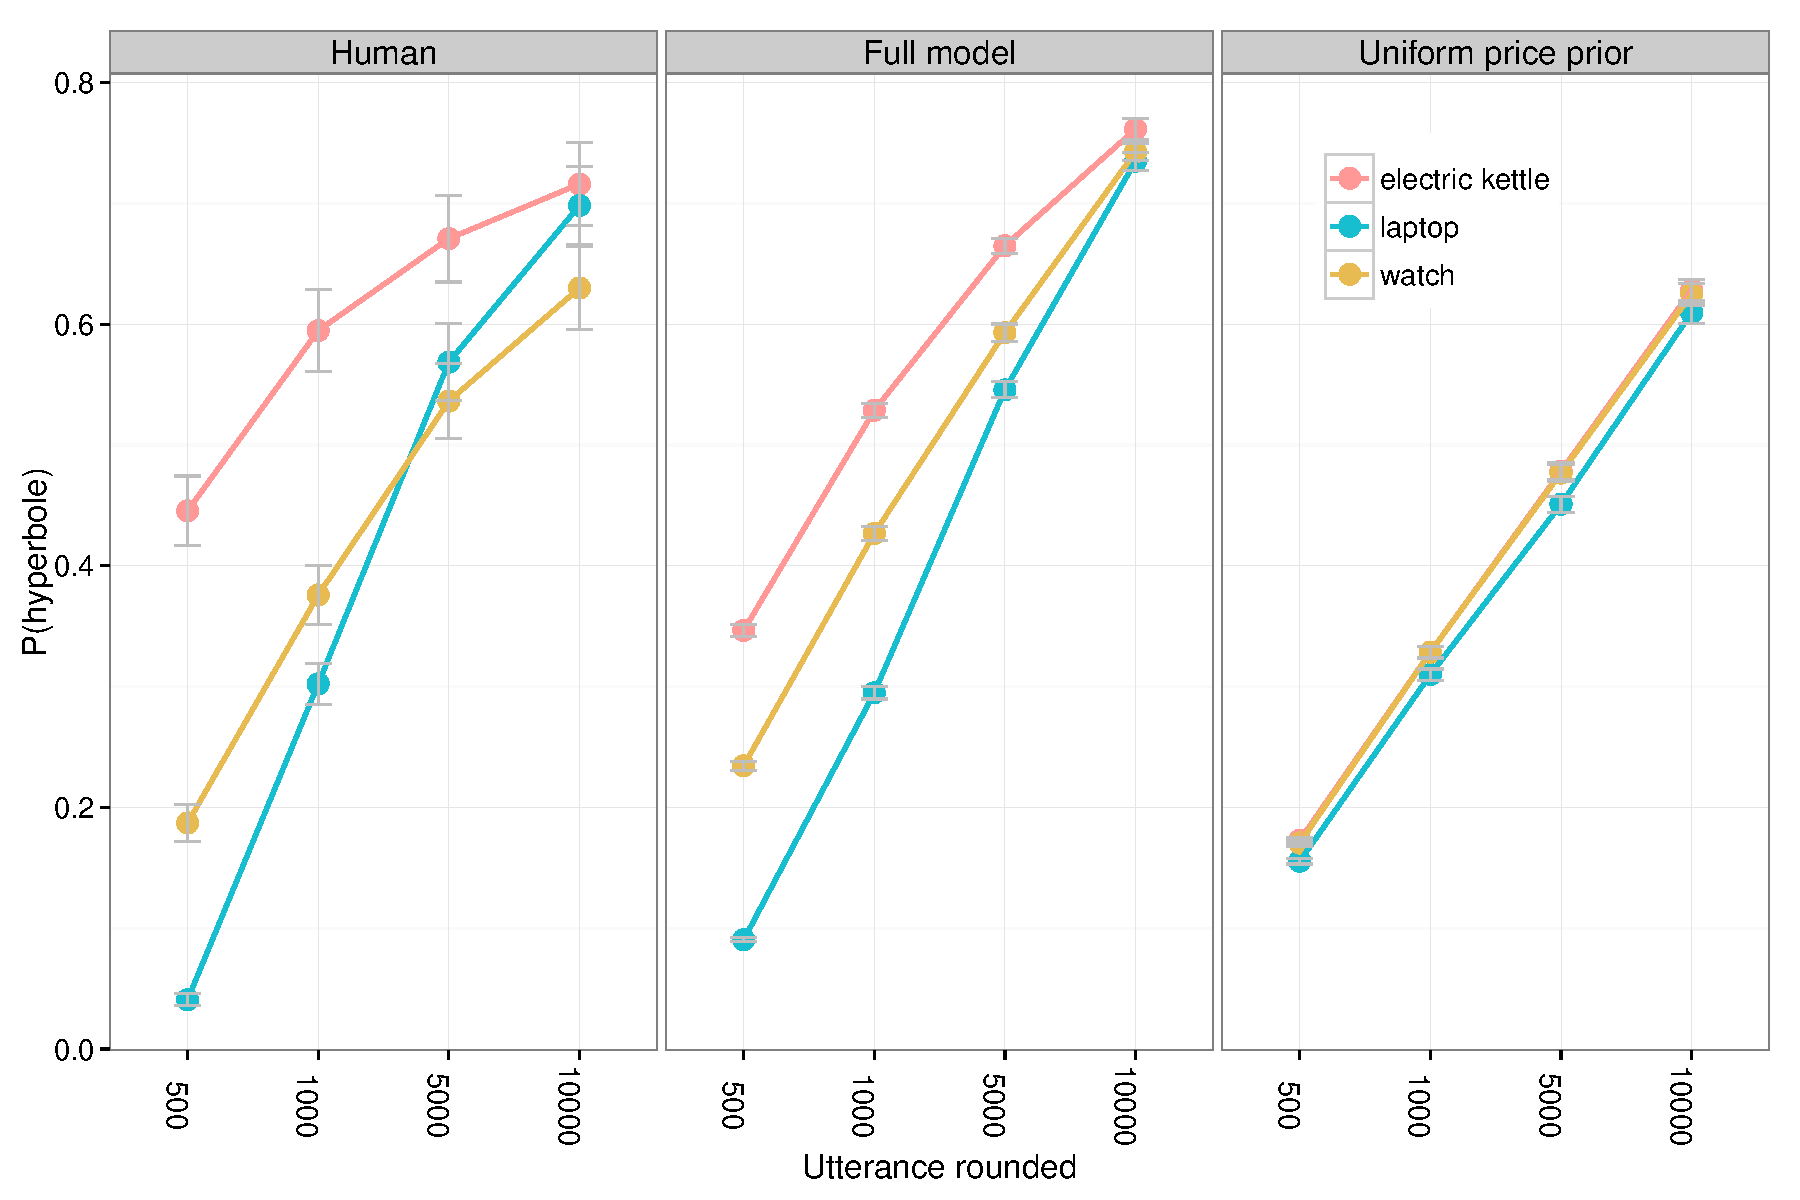
\includegraphics[width=8.7cm]{model_comp_hyperbole.pdf}
\caption{Hello}
\end{minipage}
\begin{minipage}[b]{.49\textwidth}
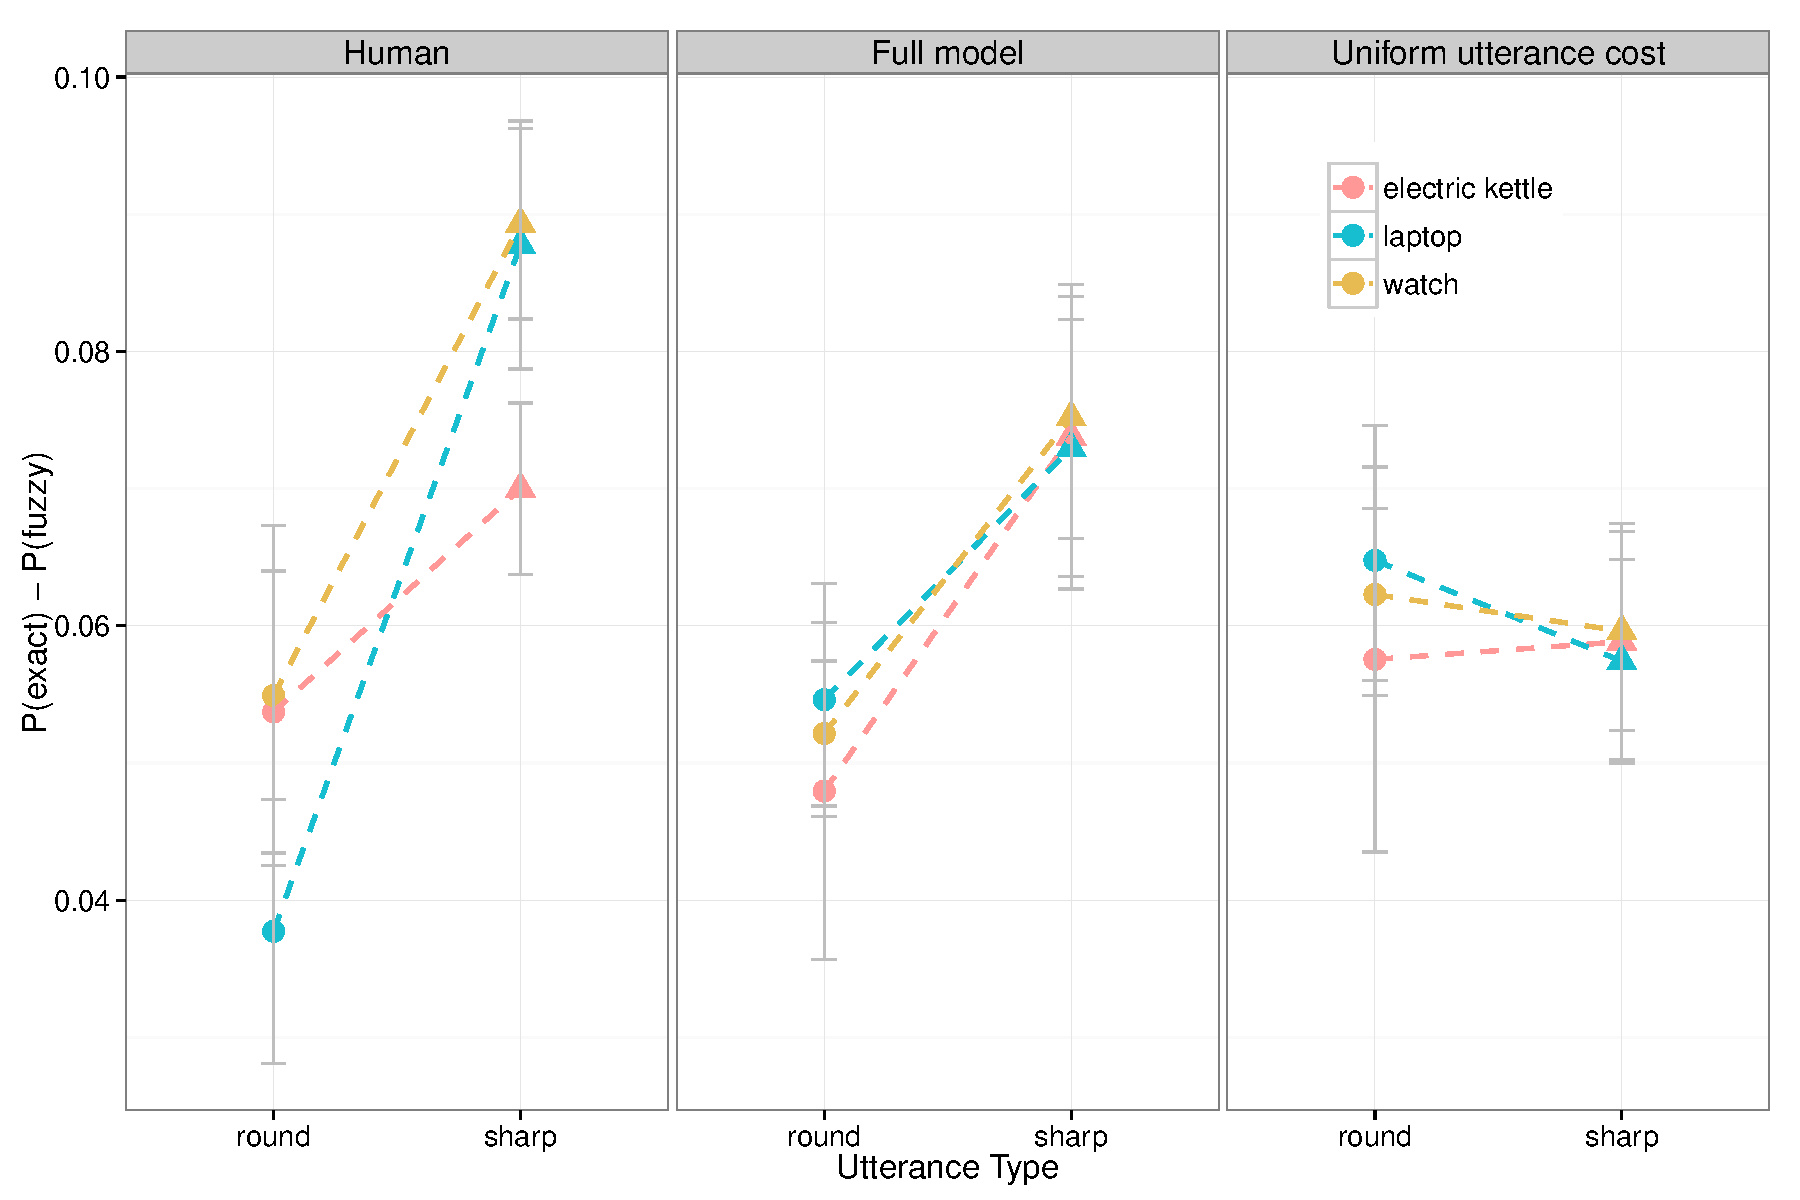
\includegraphics[width=8.7cm]{model_comp_halo.pdf}
\caption{Hello}
\end{minipage}\hfill
\caption{(A) Probability of hyperbolic interpretation across utterances and items. The leftmost panel shows human data (error bars are standard errors). A full model that uses empirical price priors matches human data; a model that uses uniform price priors does not distinguish among item types and shows weaker hyperbole effects. (B) Bias for exact interpretation for round/sharp utterance types. Humans have a bias for exact interpretations of sharp utterances. A full model that assigns higher costs to sharp numbers matches human data; a model that uses uniform utterance costs does not.}
\label{hyperbole_and_affect}
\end{figure*}

\subsection{Model simulations}

Using the price priors and affect priors measured for each of the three items, we obtained the full posterior meaning distribution predicted by the model for each utterance (see Figure \ref{full_bar}A). Figure 1 summarizes this distribution into different types of interpretations. The first three are model interpretations regarding the price state: exact (e.g.,  ``1000" interpreted as $1000$), fuzzy (e.g. ``1000" interpreted as 1001 or ``1001" interpreted as 1000), and hyperbolic (e.g. ``1000" interpreted as 100). Utterances whose literal meanings are less likely given the price prior are more likely to be interpreted hyperbolically (e.g. ``1000" is more likely to be interpreted hyperbolically for electric kettles than laptops), which captures a basic feature of hyperbole. Round utterances such as ``500" and ``1000" are interpreted less exactly and more fuzzily than their sharp counterparts, which captures pragmatic halo. On the affect dimension, affective interpretation refers to the probability that an utterance conveys the speaker's opinion that the price is expensive. Utterances whose literal meanings are associated with higher affect priors (such as ``10000" and ``10001") are more likely to be interpreted as conveying affect---predicting the affective subtext of hyperbole. 

To build intuition for these predictions, consider a pragmatic listener who recursively reasons about a speaker and analyzes her choice of utterance. The pragmatic listener hears ``10,000 dollars" and knows that its literal meaning is extremely unlikely. However, given that the speaker reasons about a literal listener who interprets ``10,000 dollars" literally and believes that the speaker very likely thinks it is expensive, ``10,000 dollars" is an  informative utterance if the speaker's goal is to communicate that the kettle is expensive (without concern for the actual price). Since the pragmatic listener uses this information to perform joint inference on the speaker's communicative goal and the meaning of the utterance, he infers that ``10,000 dollars" is likely to mean less than 10,000 dollars but that the speaker thinks it is too expensive (i.e., strong affect).
 

\subsection{Behavioral experiments}

We conducted Experiment 1 to evaluate the model's predictions for the interpreted price. Participants read scenarios in which a buyer produces an utterance about the price of an item he bought, for example: ``The electric kettle cost 1000 dollars." Participants then rate the likelihood that the item actually cost $s$ dollars for $s \in S$ (see Experiment 1 in Methods). Figure \ref{full_bar}B shows humans' interpretation distributions across all utterances. We first test the model's qualitative predictions for hyperbole and halo: Participants were more likely to interpret utterances as hyperbolic when their literal meanings have lower probabilities under the item's prior price distribution ($F(1, 10) = 44.06, p < 0.0001$). To examine the halo effect, we computed the difference between the probability of an exact interpretation and the probability of a fuzzy interpretation for each utterance. This difference is significantly smaller for round numbers than for sharp numbers ($F(1, 28)=18.94,  p < 0.001$), which indicates that round numbers tend to be interpreted less precisely than sharp numbers. To quantitatively evaluate the model's fit, we compared model and human interpretation probabilities across all utterances and showed that model predictions are highly correlated with human interpretations of number words ($r=0.974, p<0.0001$) (Figure \ref{model_fit_and_halo}A). 

To show how each component of the proposed model is necessary for capturing effects observed in the human data, we explore a series of simpler comparison models. For illustration, Figure \ref{model_fit_and_halo}B compares model interpretations of the utterance ``The electric kettle cost 1,000 dollars" given considerations of different communicative goals. A model that does not consider alternative communicative goals interprets the utterance entirely literally. A model that considers a speaker whose goal may be to communicate precisely or imprecisely interprets the utterance as meaning either 1000 or 1001. A model that considers a speaker whose goal may be to communicate the price state \emph{or} her affect prefers price states with higher prior probabilities. Finally, a model that considers the full range of goals produces interpretations that demonstrate hyperbole and halo effects that closely match humans' interpretations. This suggests that reasoning about a speaker's communicative goals is crucial for the nonliteral interpretation of number words. Figure \ref{hyperbole_and_affect}A shows probabilities of an utterance being interpreted hyperbolically by humans, the full model, and a version of the model that takes a uniform price prior for each item type. The full model faithfully captures the human data, while the ``lesioned" model fails to differentiate among hyperbole effects for the three item domains. This confirms that people rely on (common) knowledge of a domain's prior distribution to infer hyperbolic interpretations, not the semantics of the number words alone. Figure \ref{hyperbole_and_affect}B shows the halo effect in humans, the full model that assigns higher utterance costs to sharp numbers, and a version of the model where the costs of utterances are uniform. The full model replicates humans' pragmatic halo effect, while the simpler model does not. This suggests that people consider utterance costs and communicative efficiency, yielding exact versus fuzzy interpretations. 

\begin{figure*}
\centering
\begin{minipage}[b]{.49\textwidth}
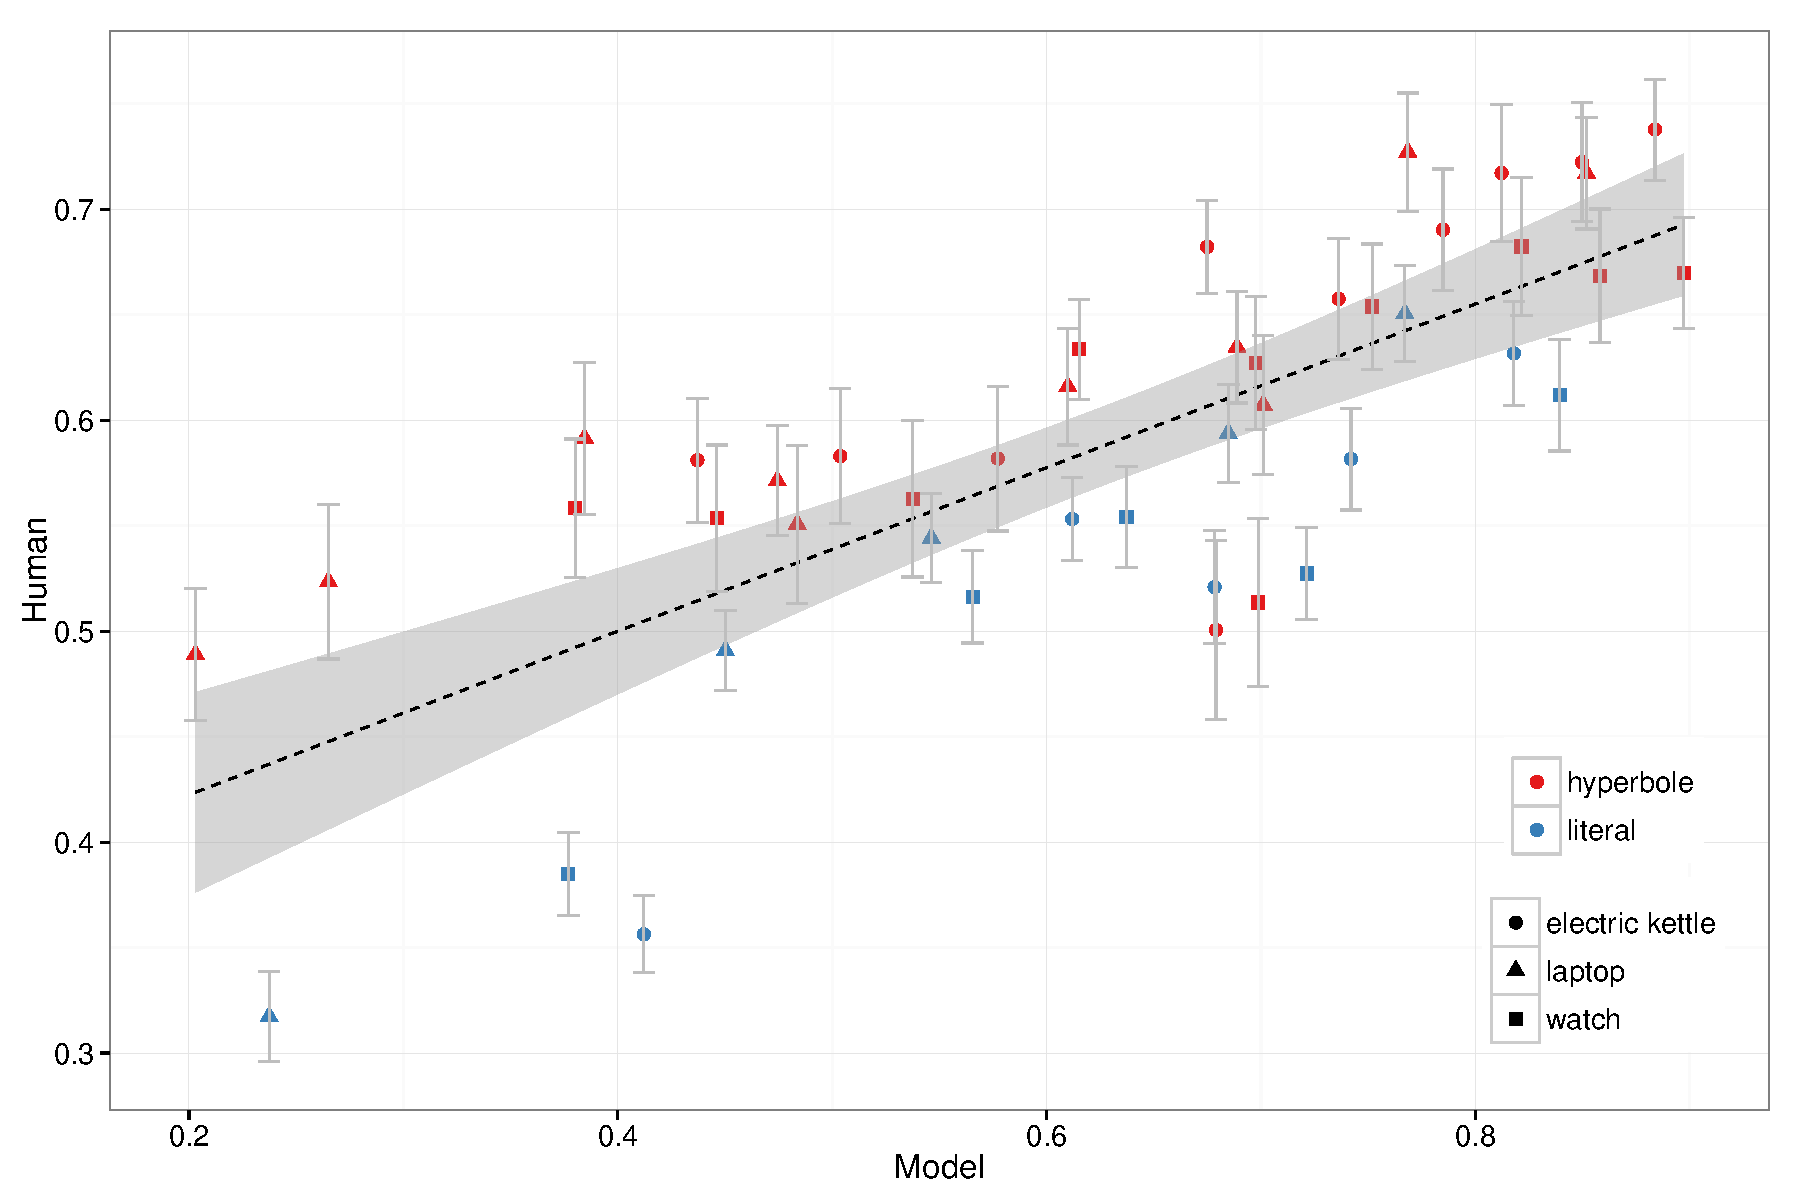
\includegraphics[width=8.7cm]{affect_scatter.pdf}
\caption{Hello}
\end{minipage}
\begin{minipage}[b]{.49\textwidth}
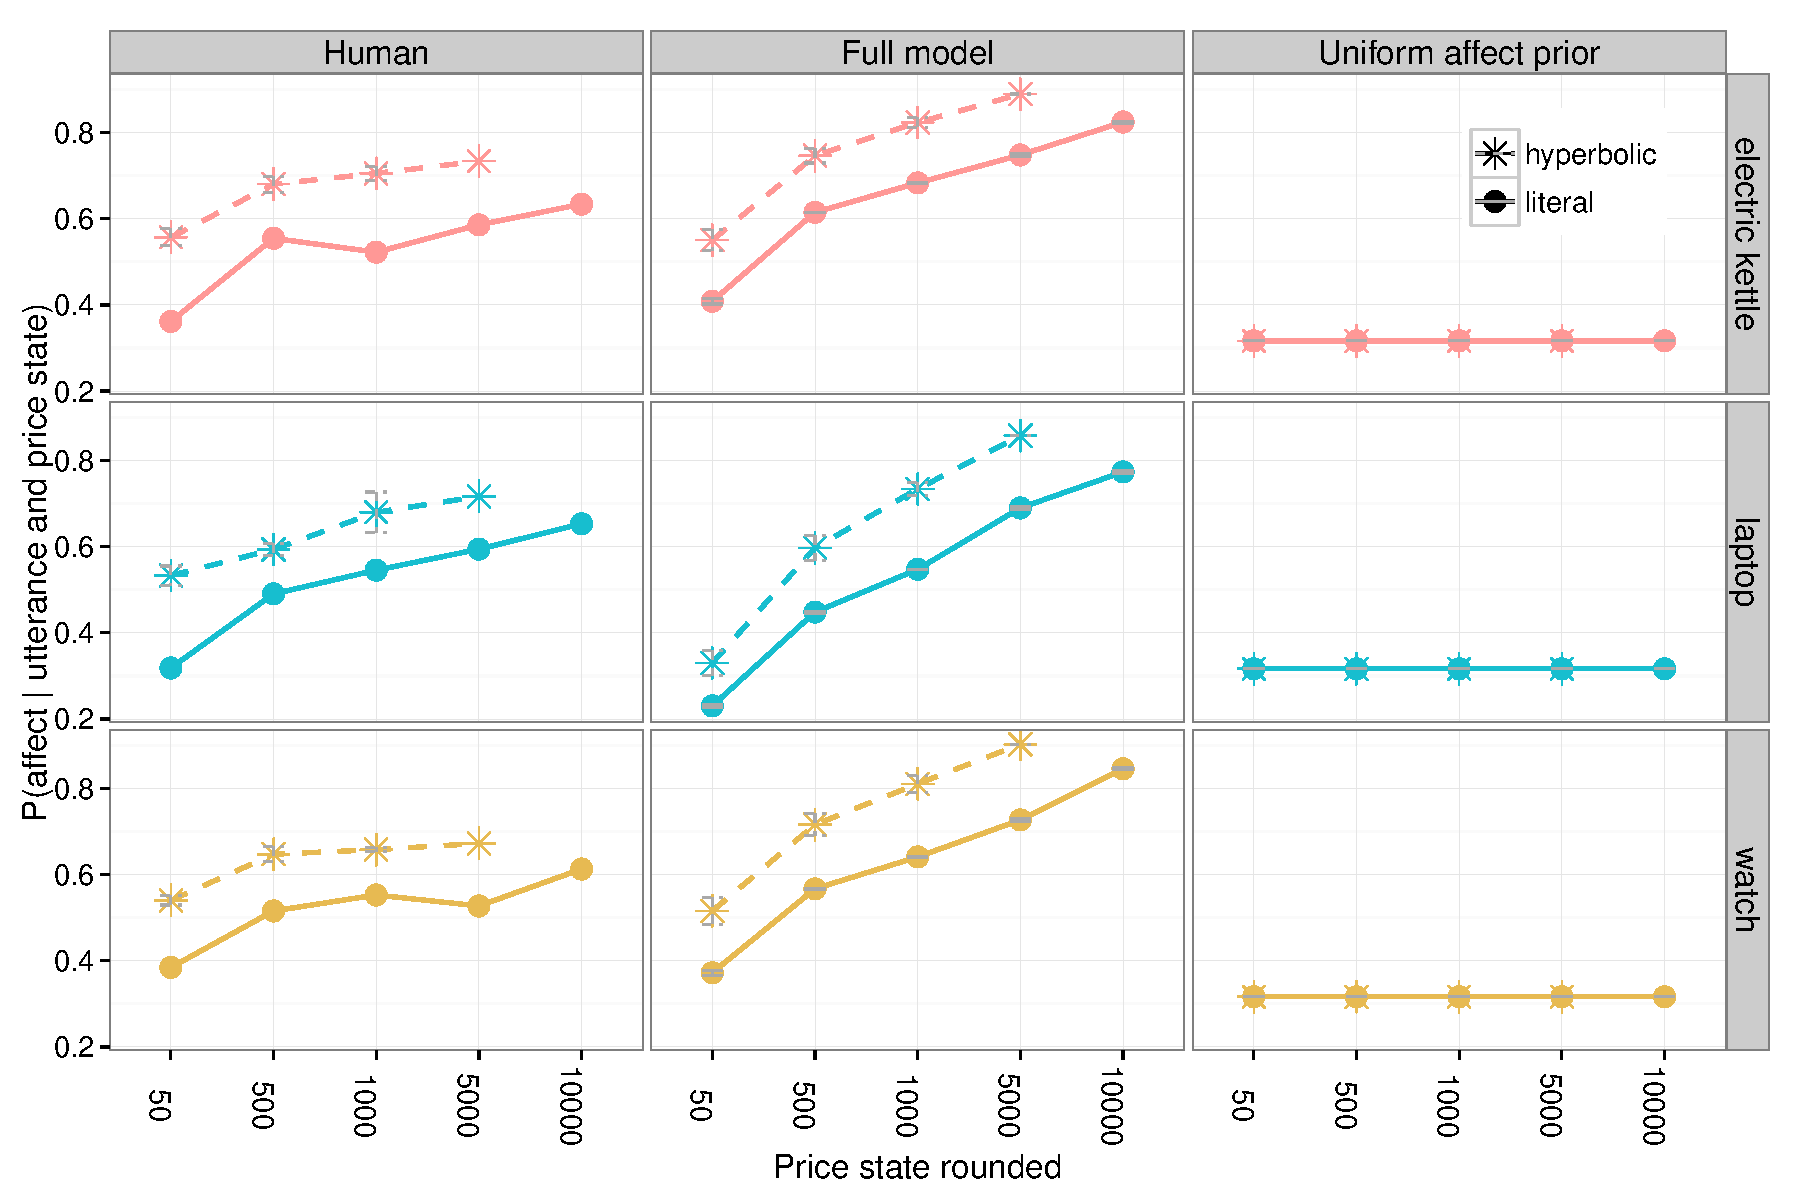
\includegraphics[width=8.7cm]{model_comp_affect.pdf}
\caption{Hello}
\end{minipage}
\caption{(A) Model predictions of affect (x-axis) versus human responses (y-axis) for 45 data points (3 Items $\times$ 15 Utterance-Price state pairs where $u \geq s$) in Experiment 2. (B) Probability of inferring affect given a price state and a hyperbolic or literal utterance. Humans infer higher probability of affect given higher price states and higher affect given hyperbolic utterances. A full model that uses empirical affect priors matches human data; a model that uses uniform affect priors predicts neither affect across price states or the rhetorical effect of hyperbole.}
\label{affect_exp}
\end{figure*}

Does the model capture the rhetorical effect of hyperbole? We conducted Experiment 2 to examine humans' inference of affect in hyperbolic versus literal utterances. Participants read scenarios in which a speaker bought an item that cost $s$ dollars and says it cost $u$ dollars, where $u \geq s$. They then rate how likely it is that the buyer thinks the item was too expensive (see Experiment 2 in Supplementary Materials). We focused on the affect of an item being too expensive due to previous findings suggesting that hyperbole is more often used to communicate negative attitudes and emotions (1, 11).  Results showed that utterances $u$ where $u > s$ are rated as significantly more likely to convey affect than utterances where $u {=} s$ ($F(1, 25)=12.57, p < 0.005$). This confirms the hypothesis that listeners infer affective subtext from hyperbolic utterances. Quantitatively, we compared model and human interpretations of affect for each of the 45 items where $u \geq s$. While there is a significant amount of noise in the human judgments (average split-half correlation is $0.833$), the model predicts human interpretations of the utterances' affective subtext significantly better than chance ($r=0.772, p < 0.00001$), capturing most of the reliable variation in these data (Figure \ref{affect_exp}A). Figure \ref{affect_exp}B shows probabilities of inferring affect given a price state and a literal or hyperbolic utterance for humans, the full model, and a version of the model that uses uniform affect priors. The human data shows that higher actual price states are associated with higher probability of affect. Within the same price state, hyperbolic utterances are interpreted as conveying more affect than literal utterances. Both effects are replicated by the full model, but not by the ``lesioned" model: the rhetorical effect of hyperbole is driven in part by prior knowledge of affect associated with different prices. 

\section{Discussion}
We have presented the first computational model of nonliteral language understanding that quantitatively predicts people's hyperbolic and imprecise interpretations of number words.  Our model and behavioral results show that complex patterns in nonliteral number interpretation depend on common ground between speaker and listener, consideration of communicative efficiency, and reasoning about relevance to the speaker's communicative goal.

The model presented here is intended to give a computational account of how people utilize prior knowledge and pragmatic reasoning to arrive at potentially nonliteral interpretations of language. However, it does not serve to predict process-level details, such as whether literal interpretations must be considered before they are rejected in favor of nonliteral interpretations. Instead, our goal was to show that formalizations of basic communicative principles---informativity with respect to a goal---can explain nonliteral language understanding as well as its rhetorical effects. We were able to examine nonliteral language at a fine-grained level and understand how the quantitative details of an utterance in context predict specific interpretations of a number word. Our model's predictions closely match humans' judgments of hyperbole, a complex phenomenon previously beyond the scope of computational models.

\hl{if there's space, would be good to include here a little about connections to informal approaches, and limitations of the current model...}

In future work, we hope to extend our model to explain nonliteral language understanding more broadly by capturing the communicative goals in other figures of speech such as irony and metaphor. We believe that this framework significantly advances the flexibility and richness of formal models of language understanding, such that some day probabilistic models will explain \emph{everything} (hyperbolically speaking). 

%----------------------------------------------------------------------------------------
%	MATERIALS AND METHODS
%----------------------------------------------------------------------------------------

%% Optional Materials and Methods Section
%% The Materials and Methods section header will be added automatically.

\begin{materials}
\section{Model}
Let $u$ be the utterance a speaker utters. The meaning of the utterance has two dimensions: the actual price state $s$ and the speaker's affect $a$. We defined the set of price states $S=\{50, 51, 500, 501, 1000, 1001, 5000, 5001, 10000, 10001\}$. We assumed that the set of utterances $U$ is identical to $S$. We defined the set of affect states $A=\{0, 1\}$ (0 means no affect and 1 means with affect). Given the price states $S$ and affect states $A$, the set of possible meanings $M$ is given by $M = S \times A$. We denote each possible meaning as $s, a$, where $s \in S$ and $a \in A$. \hl{Attempted to fix.} Let $g$ be the communicative goal, which also has two dimensions, the first concerning the price state, and the second concerning the speaker's affect. Along the price state dimension, the speaker either wants to communicate exactly, approximately, or not at all; along the affect dimension, she either wants to communicate her affect or not. Assuming that the speaker wants to communicate information on at least one dimension (otherwise she would not have produced an utterance), there are five possible goals, denoted as $g_{s, a}$, $g_{s + \eta, a}$, $g_{s}$, $g_{s+\eta}$, $g_{a}$, respectively. Formally, each goal $g$ takes in a meaning $s, a$ and projects it onto the appropriate dimension(s). We define the projection that each goal performs as the following:
%
\[\left\{ 
  \begin{array}{l l}
    g_{s,a}(s, a) =  s, a \\
    g_{s+\eta, a}(s, a) = s + \eta, a\\
    g_{s}(s, a) = s\\
    g_{s + \eta}(s, a) = s + \eta\\
    g_{a}(s, a) = a
  \end{array} \right.\]
%
where $\eta$ is a noise term that is randomly sampled from $\{-1, 0, 1\}$. 

A literal listener $L_0$ provides the base case for recursive social reasoning between the speaker and listener. $L_0$ interprets an utterance $u$ literally without taking into account the speaker's communicative goals:

%\begin{equation}\label{eq:literallistener}
%\text{
\[ L_0(s,a |u) \propto \left\{ 
  \begin{array}{l l}
    P_A(a|s) & \quad \text{if $s$ = $u$}\\
    0 & \quad \text{otherwise}
  \end{array} \right.\]
 % }
%\end{equation}
%
The speaker $S_n$ is assumed to be a rational planner who optimizes the probability that the listener will infer a meaning that satisfies her communicative goal while minimizing the cost of her utterance. $S_n$ chooses utterances according to a softmax decision rule that describes an approximately rational planner \cite{sutton1998reinforcement}:
\begin{equation}\label{eq:speakerprob}
S_n(u | s, a, g) \propto e^{ U_n(u |  s, a, g)}
\end{equation}
%
Following the Rational Speech Act model, we define the speaker�s utility as the negative surprisal of the true state under the listener�s distribution given an utterance and the negative of the utterance cost $C(u)$. However, here we assume that given a goal, the speaker only aims to maximize informativeness along the goal dimension. This leads to the following utility function for speaker $s_n$: 
\begin{equation}
U_n(u | s, a, g) = \log (\sum_{s', a'}\delta_{g(s,a)=g(s',a')}L_n(s',a'|u)) - C(u)
\end{equation}
%
Combined with equation 1, this leads to:

\begin{equation}\label{eq:speakersimplified}
S_n(u | s, a, g) \propto \sum_{s', a'}\delta_{g(s,a)=g(s',a')}L_n(s',a'|u)\cdot e^{-c(u)}
\end{equation}
%
The listener $L_n$ performs Bayesian inference to guess the intended meaning given the prior $P$ and his internal model of the speaker. To determine the speaker's intended meaning, the listener will marginalize over the possible goals under consideration.
\begin{equation}\label{eq:listenerdict}
L_n({s,a}|u) \propto \sum_{g }P_S(s)P_A(a|s)P_G(g|s,a)S_{n-1}(u | s, a, g)
\end{equation}
%
The prior probability of a price state $s$ is taken from an empirically derived price prior $P_S(s)$, and the probability of an affect $a$ given a price state $s$ is taken from an empirically derived conditional affect prior $P_A(a|s)$ (see Experiments 3a and 3b). The probability distribution $P_G(\cdot| s,a)$ over goals given that the speaker knows meaning $s, a$ is defined to be uniform over goals consistent with $s, a$. We used $C(u) = 1$ when $u$ is a round number and $C(u) = 1.8$ when $u$ is a sharp number for all model simulations reported. We obtained a posterior distribution for all possible meanings $s, a$ given an utterance $u$. Raw data for model predictions are \hl{here}: \url{http://stanford.edu/~justinek/hyperbole-paper/data/model-predictions.csv}. Figure S1 shows the full posterior distributions for all utterances.

\section{Experiment 1: Halo and hyperbole}
120 participants were recruited on Amazon's Mechanical Turk. We restricted participants to those with IP addresses in the United States. Each participant read 15 scenarios in which a person (e.g. Bob) buys an item (e.g. a watch) and is asked by a friend whether the item is expensive. We randomized the order of the trials as well as the names of the buyers. Bob responds by saying ``It cost $u$ dollars," where $u \in \{50, 50 \pm k, 500, 500 \pm k, 1000, 1000 \pm k, 5000, 5000 \pm k, 10000, 10000 \pm k\}$, where $k$ was randomly selected from the set $\{1, 2, 3\}$ for each trial. We will refer to this set of utterances as $U$. Numbers devisable by 10 are considered ``round" numbers, while numbers not devisable by 10 are ``sharp" numbers. Given an utterance $u$, participants rated the probability of Bob thinking that the item was expensive. They then rated the probability of the item costing the following amounts of money: $50, 50 \pm k, 500, 500 \pm k, 1000, 1000 \pm k, 5000, 5000 \pm k, 10000, 10000 \pm k$, where $k$ was randomly selected from the set $\{1, 2, 3\}$ for each trial. We will refer to this set of prices as $S$. Ratings for each price state were on a continuous scale from ``impossible" to ``extremely likely," represented as real values between 0 and 1. There are a total of 30 possible trial configurations (3 Items $\times$ 10 Utterances). The stimuli for Experiment 1 can be found \hl{here}: \url{http://stanford.edu/~justinek/hyperbole-paper/materials/experiment1.html}.
 
We normalized participants' ratings across price states for each trial to sum up to 1. There are a total of 300 average normalized ratings (3 Items $\times$ 10 Utterances $\times$ 10 Price States). The average normalized ratings across participants for each item/utterance pair is shown in Figure \ref{full_bar}B. The raw ratings can be found here: \url{http://stanford.edu/~justinek/hyperbole-paper/data/experiment1-raw.csv}, and the normalized ratings are here: \url{http://stanford.edu/~justinek/hyperbole-paper/data/experiment1-normalized.csv}. To adjust for humans' biases against using the extreme ends of the slider bars, we performed a power-law transformation on the model's distribution: We multiplied the predicted probability for each meaning by a free parameter $\lambda$ and renormalized the probabilities to sum up to $1$ for each utterance. Fitting $\lambda$ to the behavioral data to optimize correlation, we obtained the best fit with $\lambda=0.34$, resulting in a correlation between model predictions and participant ratings of $r = 0.974$ (see main text). All figures and analyses that we report in the main text are with this transformation. Without transformation and with no free parameters in the model, correlation between model predictions and participant ratings is still very high ($r = 0.907$).
 
For the analysis reported in Figure 3(A), we computed the probability of a participant interpreting an utterance $u$ as hyperbolic by summing up his or her probability ratings for each interpreted price state $s$, where $u>s$. Since our analysis of hyperbole does not involve utterance costs, we collapsed across round and sharp versions of utterances and price states. For example, ``1001" interpreted as 1000 does not count as hyperbole. Since 50 and 51 are the lowest available price states, the probabilities for hyperbolic interpretation of utterances ``50" and ``51" are 0. We computed the average probability of a hyperbolic interpretation across subjects for each utterance. We then showed the hyperbole effect by building a linear regression model with prior probabilities for the utterances' literal meanings as predictor and the probabilities for hyperbolic interpretation as response. Results indicated that participants were more likely to interpret utterances as hyperbolic when their literal meanings have lower probabilities under the item's prior price distribution ($F(1, 10) = 44.06, p < 0.0001$). For the analysis reported in Figure 3(B), we analyzed the pragmatic halo effect by computing each subject's bias for interpreting an utterance $u$ exactly (``1000" interpreted as 1000) versus fuzzily (``1000" interpreted as 1001). Bias was measured by subtracting the probability of a fuzzy interpretation from the probability of an exact interpretation. We then obtained the average bias for each utterance across subjects. We showed that the average bias for exact interpretation is significantly higher for sharp utterances than for round utterances ($F(1, 28)=18.94,  p < 0.001$). 

\section{Experiment 2: Affective subtext}
160 participants were recruited on Amazon's Mechanical Turk. We restricted participants to those with IP addresses in the United States. Each participant read 30 scenarios in which a person (e.g. Bob) buys an item that costs s dollars and is asked by a friend whether the item is expensive. We randomized the order of the trials as well as the names of the buyers. Bob responds by saying ``It cost $u$ dollars," where $u \in U$ and $u \geq s$. Participants then rated how likely Bob thinks the item was expensive on a continuous scale ranging from ``impossible" to ``absolutely certain," represented as real values between 0 and 1. There are a total of 180 trial configurations (3 Items $\times$ 60 $\{u, s\}$ pairs where $u\geq s$). The stimuli for Experiment 2 can be found here: \url{http://stanford.edu/~justinek/hyperbole-paper/materials/experiment2.html}; the raw data is here: \url{http://stanford.edu/~justinek/hyperbole-paper/data/experiment2-raw.csv}.

Since our analysis of affective subtext does not involve utterance cost, for the analyses reported in Figure 4(A) and 4(B), we collapsed round and sharp versions of each utterance and price state such that there are a total of 45 combinations of utterances and price states under consideration. Utterances $u$ for which $u=s$ are considered literal; utterances $u$ for which $u>s$ are hyperbolic. For the analysis reported in Figure 4(B), we obtained average ratings of affect for each utterance given that it is literal or hyperbolic. A linear regression model showed that hyperbolic utterances are rated as having significantly higher affect than literal utterances across price states ($F(1, 25) = 12.57, p < 0.005$). 

\section{Experiment 3a: Price prior}
To obtain people's prior knowledge of the price distributions for electric kettles, laptops, and watches, 30 participants were recruited from Amazon's Mechanical Turk. We restricted participants to those with IP addresses in the United States. Each participant rated the probability of an electric kettle, laptop, and watch costing $s$ dollars, where $s \in S$. We randomized the order of the trials as well as the names of the buyers. Ratings for each price state were on a continuous scale from ``impossible" to ``extremely likely," represented as real values between 0 and 1. The stimuli for Experiment 3a can be found here: \url{http://stanford.edu/~justinek/hyperbole-paper/materials/experiment3a.html}. We normalized participants' ratings across price points for each trial to sum up to 1. The average normalized ratings across participants for each item were taken as the prior probability distribution of item prices. These price distributions were used in the model to determine the prior probability of each price state. The normalized ratings can be found here: \url{http://stanford.edu/~justinek/hyperbole-paper/data/experiment3a-normalized.csv}

\section{Experiment 3b: Affect prior}
To obtain people's prior knowledge of the affect likelihood given a price state, 30 participants were recruited from Amazon's Mechanical Turk. We restricted participants to those with IP addresses in the United States. Each participant read 15 scenarios where someone had just bought an item that cost s dollars ($s \in S$). We randomized the order of the trials. They then rated how likely the buyer thinks the item was expensive on a continuous scale ranging from ``impossible" to ``absolutely certain," represented as real values between 0 and 1. The stimuli for Experiment 3b can be found here: \url{http://stanford.edu/~justinek/hyperbole-paper/materials/experiment3b.html}. The average ratings for each item/price state pair were taken as the prior probability of an affect given a price state. This was used in the model to determine the prior probability of an affect given each price state. The data can be found here: \url{http://stanford.edu/~justinek/hyperbole-paper/data/experiment3b-raw.csv} 

\begin{figure*}[tbh]
\label{full_bar}
\centering
\begin{minipage}[b]{.49\textwidth}
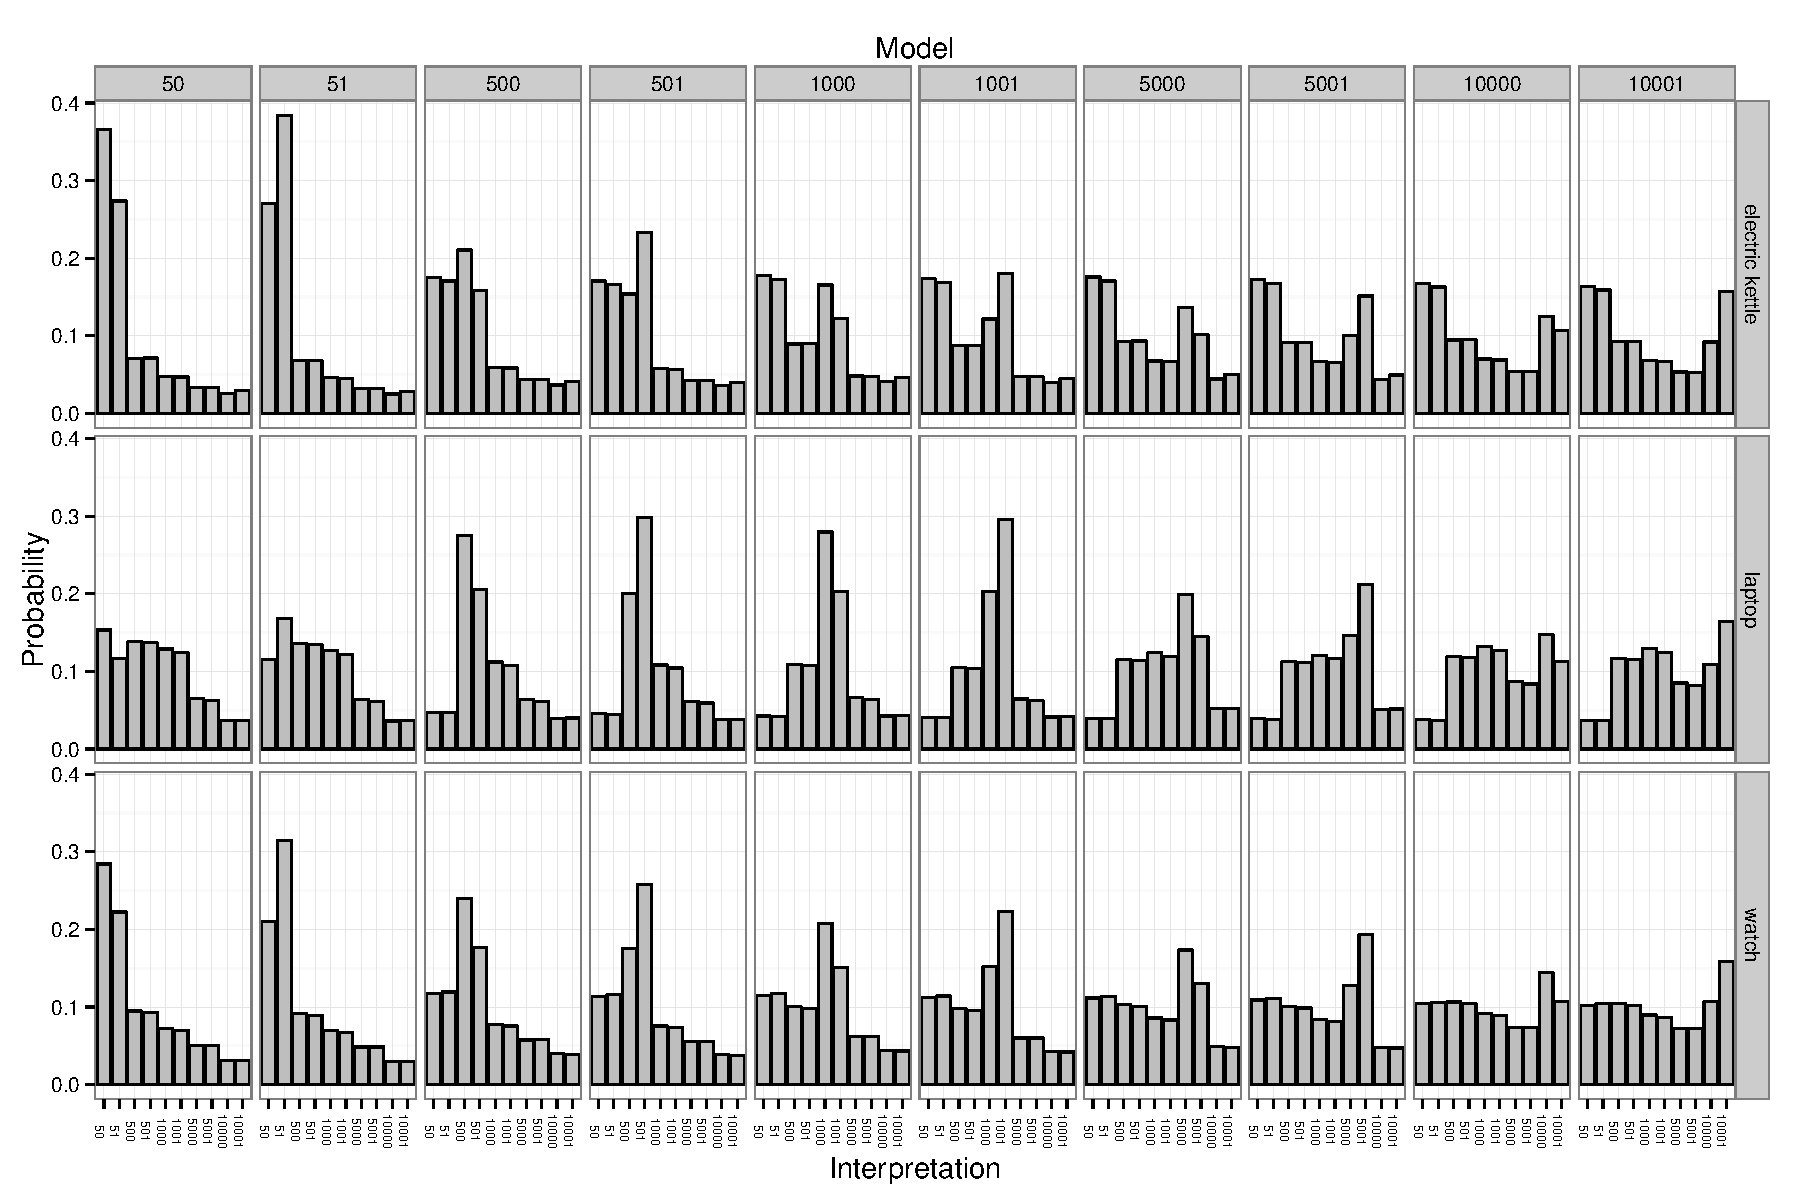
\includegraphics[width=9cm]{model_bar.pdf}
\end{minipage}
\begin{minipage}[b]{.49\textwidth}
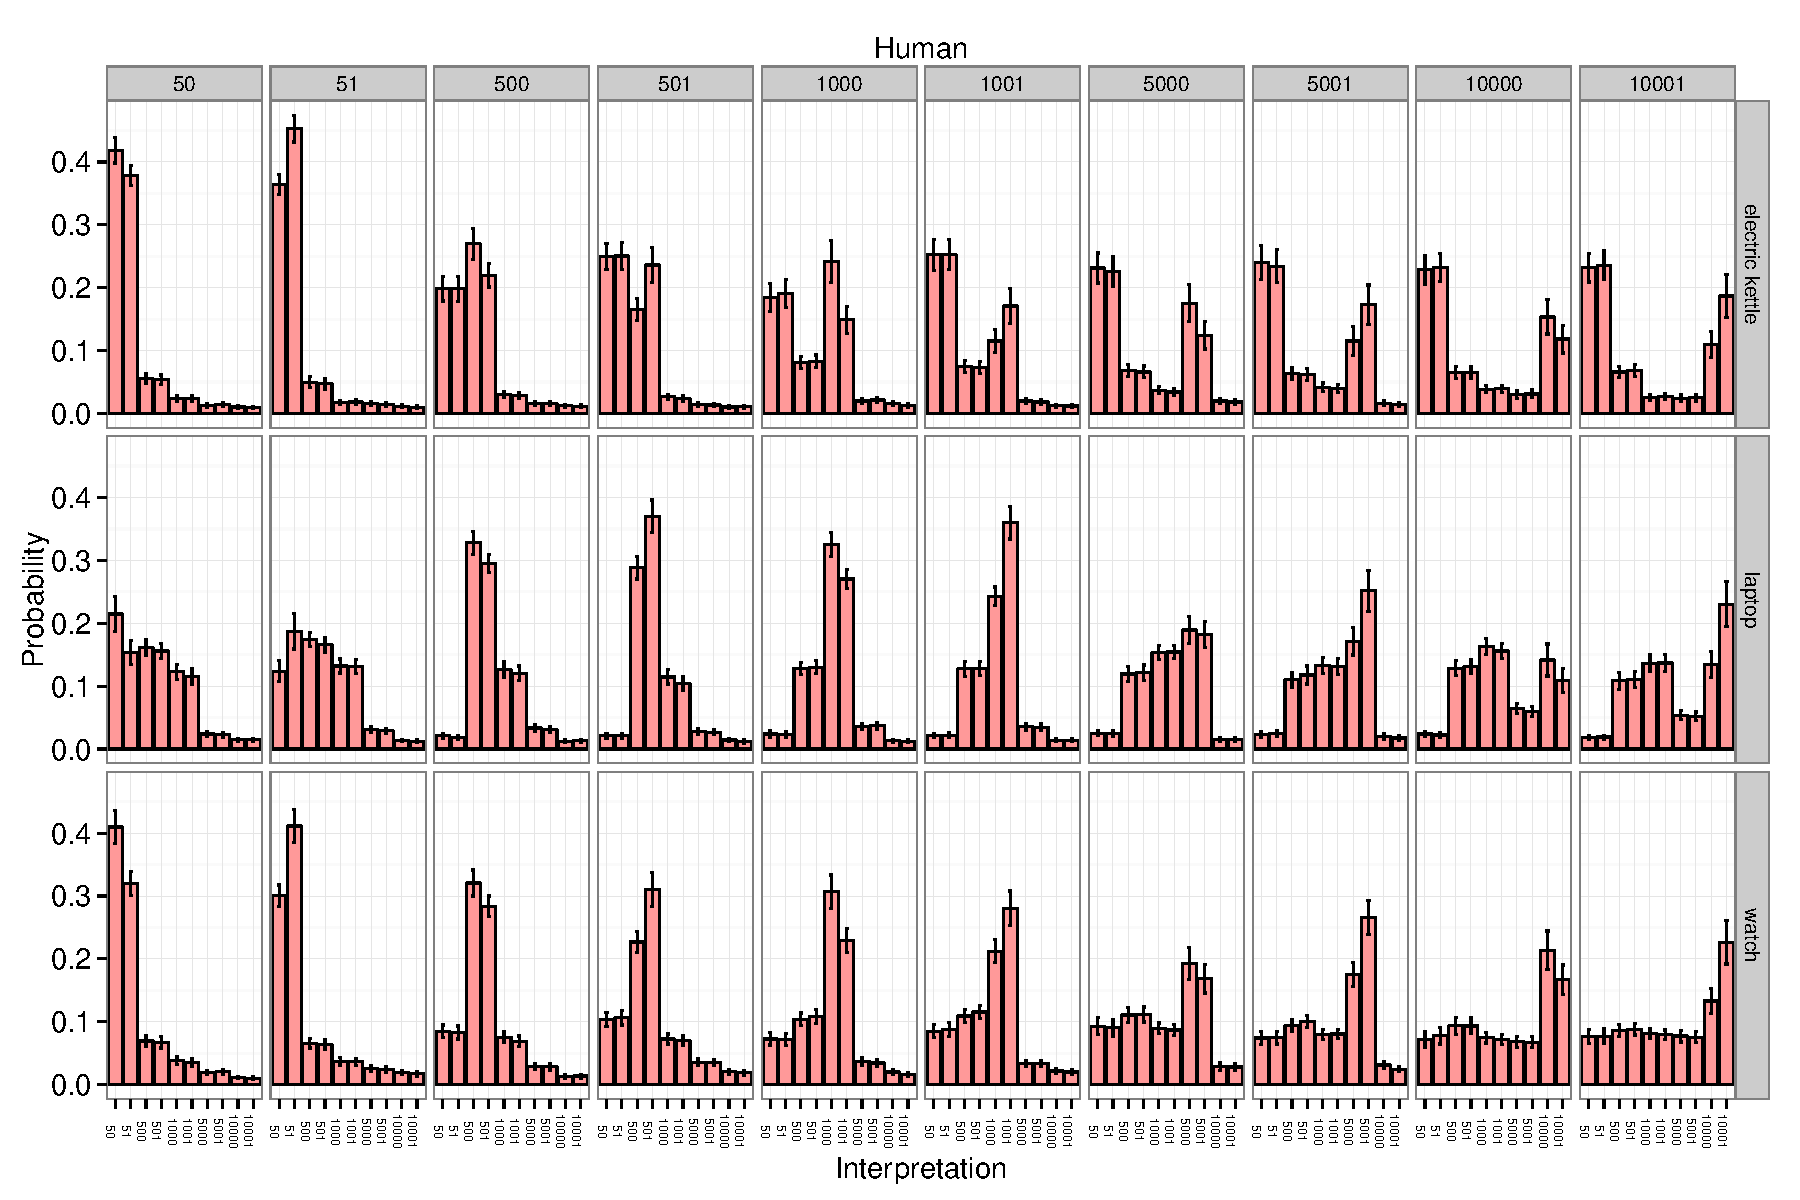
\includegraphics[width=9cm]{human_bar.pdf}
\end{minipage}
\caption{(A)Full posterior meaning distribution predicted by the model for each utterance. Each column of panels is an utterance, and each row of panels is an item type. Each panel represents the interpretation distribution given an utterance for an item. (B) Full meaning distribution produced by humans for each utterance. Each column of panels is an utterance, and each row is an item type. Each panel represents the interpretation distribution given an utterance for an item. Error bars are standard errors.}
\end{figure*}


\end{materials}

%----------------------------------------------------------------------------------------
%	APPENDICES (OPTIONAL)
%----------------------------------------------------------------------------------------

%\appendix[Appendix title]

%\begin{figure*}[h]
%\centering
%\begin{minipage}[b]{.49\textwidth}
%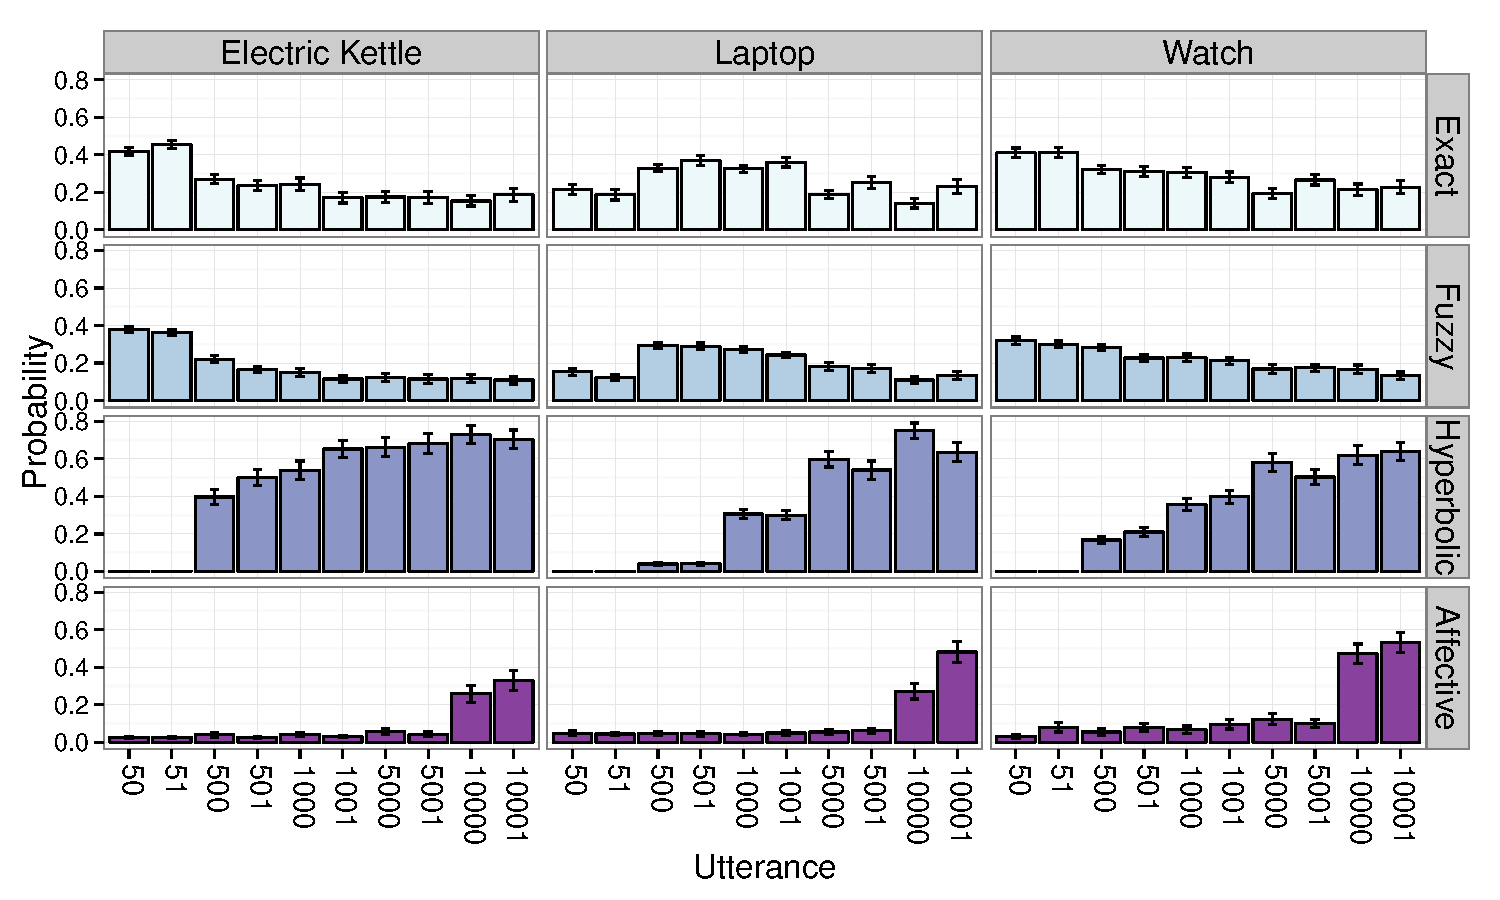
\includegraphics[width=8.7cm]{human_effect_bar.pdf}
%\caption{Hello}\label{model_effects}
%\end{minipage}\hfill
%\begin{minipage}[b]{.49\textwidth}
%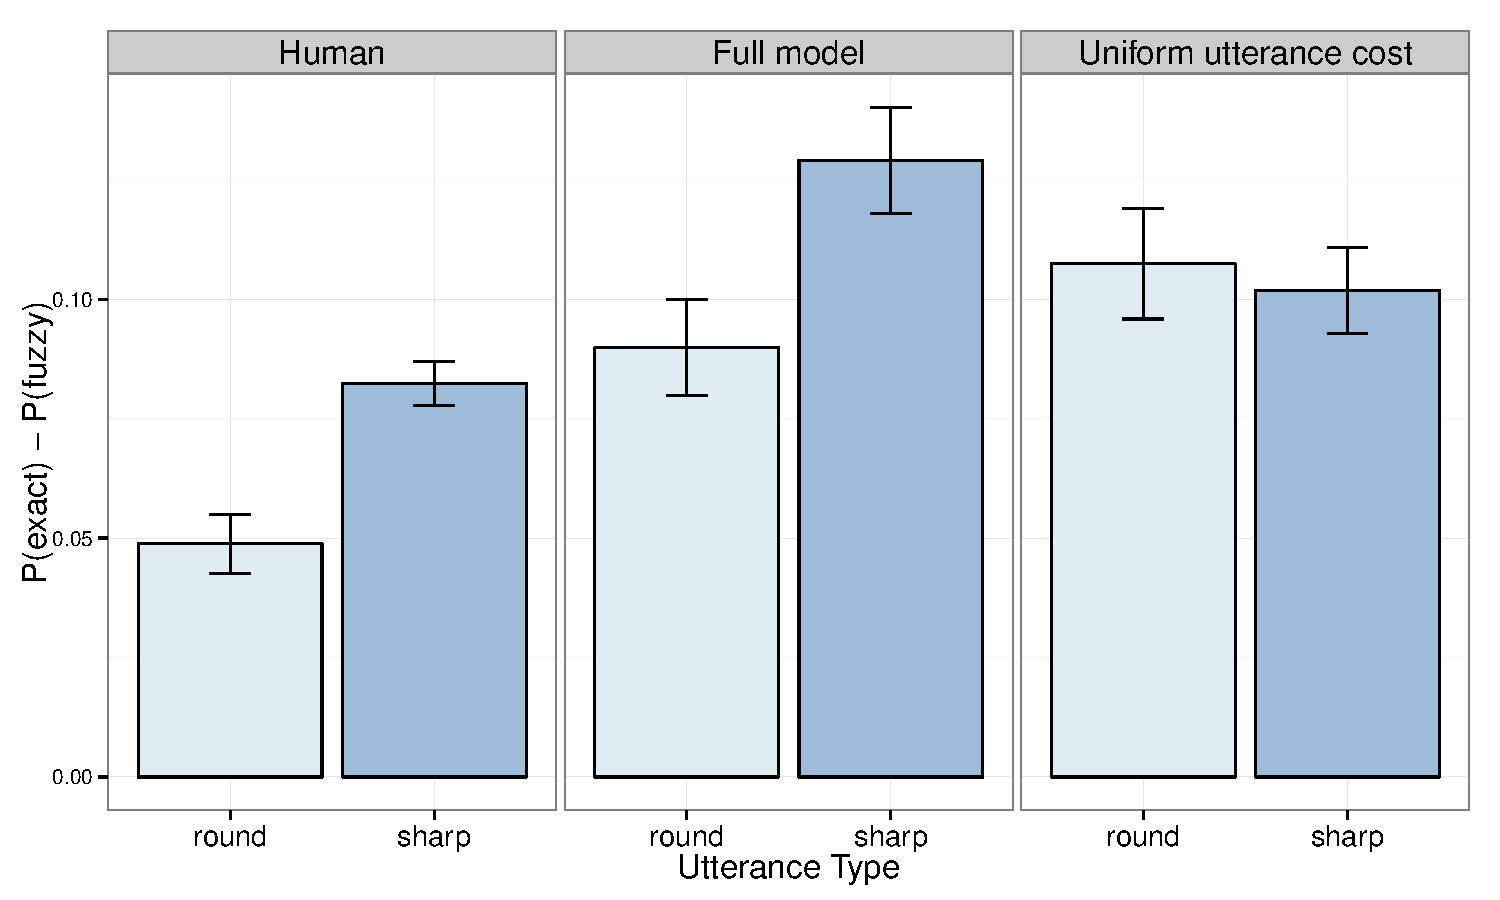
\includegraphics[width=8.7cm]{halo_comp.pdf}
%\caption{Vertical panels show results for the three item kinds. Horizontal panels show the three kinds of interpretations, \emph{exact}, \emph{fuzzy}, and \emph{hyperbolic}. The $x$ axis in each panel represents the utterance. The $y$ axis shows the probability of a kind of interpretation given the utterance.}\label{human_effects}
%\end{minipage}
%\end{figure*}

%%%%
% QUESTION: Not sure if we want this table....
%%%
%\begin{table}
%\begin{tabular}{l l}
%\hline
%\textbf{Model} & \textbf{Fit ($R^2$)}\\
%\hline
%Full & $0.938$\\
%Uniform prior & 0.560 \\
%Uniform cost & 0.939 \\
%Uniform affect & 0.921 \\
%No valence goal & 0.144 \\
%No imprecision goal & 0.726 \\
%\hline
%\end{tabular}
%\label{model_fit}
%\end{table}


%----------------------------------------------------------------------------------------
%	ACKNOWLEDGEMENTS
%----------------------------------------------------------------------------------------

\begin{acknowledgments}
Thanks!
\end{acknowledgments}

%----------------------------------------------------------------------------------------
%	BIBLIOGRAPHY
%----------------------------------------------------------------------------------------

%% PNAS does not support submission of supporting .tex files such as BibTeX.
%% Instead all references must be included in the article .tex document. 
%% If you currently use BibTeX, your bibliography is formed because the 
%% command \verb+\bibliography{}+ brings the <filename>.bbl file into your
%% .tex document. To conform to PNAS requirements, copy the reference listings
%% from your .bbl file and add them to the article .tex file, using the
%% bibliography environment described above.  

%%  Contact pnas@nas.edu if you need assistance with your
%%  bibliography.

% Sample bibliography item in PNAS format:
%% \bibitem{in-text reference} comma-separated author names up to 5,
%% for more than 5 authors use first author last name et al. (year published)
%% article title  {\it Journal Name} volume #: start page-end page.
%% ie,
% \bibitem{Neuhaus} Neuhaus J-M, Sitcher L, Meins F, Jr, Boller T (1991) 
% A short C-terminal sequence is necessary and sufficient for the
% targeting of chitinases to the plant vacuole. 
% {\it Proc Natl Acad Sci USA} 88:10362-10366.


%% Enter the largest bibliography number in the facing curly brackets
%% following \begin{thebibliography}

\begin{thebibliography}{10}

%\bibitem{moreno2007creativity}
%Moreno, R.E.V.,
%{\em Creativity and convention: The pragmatics of everyday figurative speech},
%156, (2007)

\bibitem{roberts1994}
Roberts, R.M. and Kreuz, R.J., {\em Why do people use figurative language?}, (1994), Psychological Science. 5(3), pp. ~159--163

\bibitem{dews1999}
Dews, S. and Winner, E. {\em Obligatory processing of literal and nonliteral meanings in verbal irony}, (1999), Journal of Pragmatics. 31(12), pp~1579--1599.

\bibitem{glucksberg2001}
Glucksberg, S. {\em Understanding figurative language: From metaphors to idioms}, (2001), Oxford Univ. Press.

\bibitem{gibbs1999}
Gibbs, R. {\em Figurative language}, (1999), The MIT encyclopedia of the cognitive sciences, pp.~314--315.

\bibitem{grice1975}
Grice, H.P. {\em Logic and conversation}, (1975), pp.~41--58.

\bibitem{clark1996}
Clark, H.H. {\em Using language} (1996) Cambridge University Press, Vol. 4

\bibitem{relevance}
Sperber, D. and Wilson, D. and Ziran, H. {\em Relevance: Communication and cognition}, (1986).

\bibitem{wilson2002}
Wilson, D. and Sperber, D. {\em Relevance theory}, (2002), Handbook of pragmatics.

\bibitem{sperber2008}
Sperber, D., and Wilson, D. {\em A deflationary account of metaphors}, (2008), The Cambridge handbook of metaphor and thought, pp.~84--105.

\bibitem{wilson2006}
Wilson, D. and Carston, R. {\em Metaphor, relevance and the �emergent property' issue}, (2006), Mind and Language, 21(3), pp.~404--433.

\bibitem{loosetalk}
Sperber, D. and Wilson, D. {\em Loose talk}, (1985), In Proceedings of the Aristotelian society, pp.~153--171.

\bibitem{frankgoodmanscience}
Frank, M.C. and Goodman, N.D.,
{\em Predicting pragmatic reasoning in language games},
Science, 336(6048), (2012), pp.~998

\bibitem{goodmanstuhlmueller}
Goodman, N.D. and Stuhlm{\"u}ller, A.
{\em Knowledge and implicature: Modeling language understanding as social cognition},
Proceedings of CogSci conference, (2012)

\bibitem{bergen2012}
Bergen, L. and Goodman, G.D. and Levy, R.,
{\em That's what she (could have) said: How alternative utterances affect language use},
Proceedings of CogSci conference, (2012)

\bibitem{jager2009pragmatic}
J{\"a}ger, G. and Ebert, C.,
{\em Pragmatic rationalizability},
Proceedings of Sinn und Bedeutung, 13, (2009), pp.~1--15

\bibitem{mccarthy2004there}
McCarthy, M. and Carter, R, {\em There's millions of them: hyperbole in everyday conversation},
Journal of pragmatics, 36(2), (2004), pp.~149--184.

\bibitem{gibbs2000irony}
Gibbs, R.W.,
{\em Irony in talk among friends},
Metaphor and symbol, (2000), pp.~5--27

\bibitem{gibbs1991}
Gibbs, R.W. and O'Brien J., {\em Psychological aspects of irony understanding}, Journal of pragmatics,16(6), (1991), pp.~523--530

\bibitem{lasersohn1999}
Lasersohn, P., {\em Pragmatic halos}, Language, (1991), pp.~522--551

\bibitem{bastiaanse2011rationality}
Bastiaanse, H.,
{\em The rationality of round interpretation},
Vagueness in communication, (2011), pp.~37--50

\bibitem{krifka2007approximate}
Krifka, M.,
{\em Approximate interpretation of number words: A case for strategic communication},
Cognitive foundations of interpretation, (2007), pp.~111--126

\bibitem{vanderhest2002}
Van der Henst, J. and Carles, L. and Sperber, D. {\em Truthfulness and Relevance in Telling the Time}, Mind and Language, (2002), 17(5)

\bibitem{sutton1998reinforcement}
Sutton, R.S. and Barto, A.G.,
{\em Reinforcement learning: An introduction},
28, (1998)
%	

%	}
%	
%	
%	@article{kotthoff2003responding,
%	  title={Responding to irony in different contexts: On cognition in conversation},
%	  author={Kotthoff, H.},
%	  journal={Journal of pragmatics},
%	  volume={35},
%	  number={9},
%	  pages={1387--1411},
%	  year={2003},
%	  publisher={Elsevier}
%	}
%	
%	@article{kreuz2000production,
%	  title={The production and processing of verbal irony},
%	  author={Kreuz, R.J.},
%	  journal={Metaphor and Symbol},
%	  volume={15},
%	  number={1-2},
%	  pages={99--107},
%	  year={2000},
%	  publisher={Taylor \& Francis}
%	}
%	
%	@article{kreuz1995two,
%	  title={Two cues for verbal irony: Hyperbole and the ironic tone of voice},
%	  author={Kreuz, R.J. and Roberts, R.M.},
%	  journal={Metaphor and symbol},
%	  volume={10},
%	  number={1},
%	  pages={21--31},
%	  year={1995},
%	  publisher={Taylor \& Francis}
%	}
%	
%	@article{capelli1990children,
%	  title={How children understand sarcasm: The role of context and intonation},
%	  author={Capelli, C.A. and Nakagawa, N. and Madden, C.M.},
%	  journal={Child Development},
%	  volume={61},
%	  number={6},
%	  pages={1824--1841},
%	  year={1990},
%	  publisher={Wiley Online Library}
%	}
%	

%	

%	


\end{thebibliography}

%	
%	
%	
%	@inproceedings{stiller2011ad,
%	  title={Ad-hoc scalar implicature in adults and children},
%	  author={Stiller, A. and Goodman, N.D. and Frank, M.C.},
%	  booktitle={Proceedings of the 33rd Annual Meeting of the Cognitive Science Society},
%	  year={2011}
%	}
%	
%	
%	@inproceedings{sauerland2007scalar,
%	  title={Scalar vs. epistemic vagueness: Evidence from approximators},
%	  author={Sauerland, U. and Stateva, P.},
%	  booktitle={Proceedings of SALT},
%	  volume={17},
%	  number={0},
%	  pages={228--245},
%	  year={2007}
%	}
%	
%	
%	@article{van2004signalling,
%	  title={Signalling games select Horn strategies},
%	  author={{van Rooij}, R.},
%	  journal={Linguistics and Philosophy},
%	  volume={27},
%	  number={4},
%	  pages={493--527},
%	  year={2004},
%	  publisher={Springer}
%	}
%	
%	@article{van2008games,
%	  title={Games and Quantity implicatures},
%	  author={{van Rooij}, R.},
%	  journal={Journal of Economic Methodology},
%	  volume={15},
%	  number={3},
%	  pages={261--274},
%	  year={2008},
%	  publisher={Taylor \& Francis}
%	}
%	
%	@article{franke2009interpretation,
%	  title={Interpretation of optimal signals},
%	  author={Franke, M.},
%	  journal={New perspectives on games and interaction},
%	  pages={297--310},
%	  year={2009},
%	  publisher={Amsterdam University Press}
%	}
%	
%	

%	

%	
%	@article{jager2008game,
%	  title={Game theory in semantics and pragmatics},
%	  author={J{\"a}ger, G.},
%	  journal={manuscript, University of Bielefeld},
%	  year={2008}
%	}
%	
%	@article{cho1987signaling,
%	  title={Signaling games and stable equilibria},
%	  author={Cho, I.K. and Kreps, D.M.},
%	  journal={The Quarterly Journal of Economics},
%	  volume={102},
%	  number={2},
%	  year={1987},
%	  publisher={Oxford University Press}
%	}
%	
%	@article{chen2008selecting,
%	  title={Selecting Cheap-Talk Equilibria},
%	  author={Chen, Y. and Kartik, N. and Sobel, J.},
%	  journal={Econometrica},
%	  volume={76},
%	  number={1},
%	  pages={117--136},
%	  year={2008},
%	  publisher={Wiley Online Library}
%	}
%	

%	
%	

%	
%	
%----------------------------------------------------------------------------------------

\end{article}

%----------------------------------------------------------------------------------------
%	FIGURES AND TABLES
%----------------------------------------------------------------------------------------

%% Adding Figure and Table References
%% Be sure to add figures and tables after \end{article}
%% and before \end{document}

%% For figures, put the caption below the illustration.
%%
%% \begin{figure}
%% \caption{Almost Sharp Front}\label{afoto}
%% \end{figure}

%% For Tables, put caption above table
%%
%% Table caption should start with a capital letter, continue with lower case
%% and not have a period at the end
%% Using @{\vrule height ?? depth ?? width0pt} in the tabular preamble will
%% keep that much space between every line in the table.

%% \begin{table}
%% \caption{Repeat length of longer allele by age of onset class}
%% \begin{tabular}{@{\vrule height 10.5pt depth4pt  width0pt}lrcccc}
%% table text
%% \end{tabular}
%% \end{table}

%% For two column figures and tables, use the following:

%% \begin{figure*}
%% \caption{Almost Sharp Front}\label{afoto}
%% \end{figure*}

%% \begin{table*}
%% \caption{Repeat length of longer allele by age of onset class}
%% \begin{tabular}{ccc}
%% table text
%% \end{tabular}
%% \end{table*}

%----------------------------------------------------------------------------------------

\end{document}